%% knit("our_lass_report_analysis.Rnw")

\documentclass[12pt]{article}\usepackage[]{graphicx}\usepackage[]{color}
%% maxwidth is the original width if it is less than linewidth
%% otherwise use linewidth (to make sure the graphics do not exceed the margin)
\makeatletter
\def\maxwidth{ %
  \ifdim\Gin@nat@width>\linewidth
    \linewidth
  \else
    \Gin@nat@width
  \fi
}
\makeatother

\definecolor{fgcolor}{rgb}{0.345, 0.345, 0.345}
\newcommand{\hlnum}[1]{\textcolor[rgb]{0.686,0.059,0.569}{#1}}%
\newcommand{\hlstr}[1]{\textcolor[rgb]{0.192,0.494,0.8}{#1}}%
\newcommand{\hlcom}[1]{\textcolor[rgb]{0.678,0.584,0.686}{\textit{#1}}}%
\newcommand{\hlopt}[1]{\textcolor[rgb]{0,0,0}{#1}}%
\newcommand{\hlstd}[1]{\textcolor[rgb]{0.345,0.345,0.345}{#1}}%
\newcommand{\hlkwa}[1]{\textcolor[rgb]{0.161,0.373,0.58}{\textbf{#1}}}%
\newcommand{\hlkwb}[1]{\textcolor[rgb]{0.69,0.353,0.396}{#1}}%
\newcommand{\hlkwc}[1]{\textcolor[rgb]{0.333,0.667,0.333}{#1}}%
\newcommand{\hlkwd}[1]{\textcolor[rgb]{0.737,0.353,0.396}{\textbf{#1}}}%

\usepackage{framed}
\makeatletter
\newenvironment{kframe}{%
 \def\at@end@of@kframe{}%
 \ifinner\ifhmode%
  \def\at@end@of@kframe{\end{minipage}}%
  \begin{minipage}{\columnwidth}%
 \fi\fi%
 \def\FrameCommand##1{\hskip\@totalleftmargin \hskip-\fboxsep
 \colorbox{shadecolor}{##1}\hskip-\fboxsep
     % There is no \\@totalrightmargin, so:
     \hskip-\linewidth \hskip-\@totalleftmargin \hskip\columnwidth}%
 \MakeFramed {\advance\hsize-\width
   \@totalleftmargin\z@ \linewidth\hsize
   \@setminipage}}%
 {\par\unskip\endMakeFramed%
 \at@end@of@kframe}
\makeatother

\definecolor{shadecolor}{rgb}{.97, .97, .97}
\definecolor{messagecolor}{rgb}{0, 0, 0}
\definecolor{warningcolor}{rgb}{1, 0, 1}
\definecolor{errorcolor}{rgb}{1, 0, 0}
\newenvironment{knitrout}{}{} % an empty environment to be redefined in TeX

\usepackage{alltt}
\usepackage{times}
\usepackage{hyperref}
\usepackage{natbib}
\usepackage{fullpage}
\usepackage{pdflscape}
\hypersetup{pdfpagemode=UseNone} % don't show bookmarks on initial view
\hypersetup{colorlinks, urlcolor={blue}}

% revise margins
\setlength{\headheight}{0.0in}
\setlength{\topmargin}{0.0in}
\setlength{\headsep}{0.0in}
\setlength{\textheight}{8.65in}
\setlength{\footskip}{0.35in}
\setlength{\oddsidemargin}{0.0in}
\setlength{\evensidemargin}{0.0in}
\setlength{\textwidth}{6.5in}

\setlength{\parskip}{6pt}
\setlength{\parindent}{0pt}

\title{\emph{Our Lass} 70mm versus 80mm analysis}
\author{For discussion}
\date{}
\IfFileExists{upquote.sty}{\usepackage{upquote}}{}
\begin{document}



\maketitle

\section{Data}

Read the data in and make a few factor variables
\begin{knitrout}\footnotesize
\definecolor{shadecolor}{rgb}{0.969, 0.969, 0.969}\color{fgcolor}\begin{kframe}
\begin{alltt}
\hlkwd{library}\hlstd{(gdata)}
\hlkwd{library}\hlstd{(reshape)}

\hlstd{neph.dat} \hlkwb{<-} \hlkwd{read.xls}\hlstd{(}\hlstr{"../data/2015 BIM Nephrops quad rig trials/Our Lass 2 70_80_90_100mm codends Irish Sea July 2015/Nephrops Raised Counts Our Lass 2 Irish Sea July 2015.xlsx"}\hlstd{,}
                     \hlkwc{sheet} \hlstd{=} \hlstr{"All hauls"}\hlstd{,}
                     \hlkwc{stringsAsFactors} \hlstd{=} \hlnum{FALSE}\hlstd{)}

\hlcom{## subset containing the 70mm and 80mm data}
\hlstd{neph.7080} \hlkwb{<-} \hlkwd{subset}\hlstd{(neph.dat, Mesh.Size} \hlopt \hlkwd{c}\hlstd{(}\hlstr{"70mm"}\hlstd{,} \hlstr{"80mm"}\hlstd{))}

\hlcom{## make factor haul variable}
\hlstd{neph.7080}\hlopt{$}\hlstd{fHAUL} \hlkwb{<-} \hlkwd{factor}\hlstd{(}\hlkwd{paste}\hlstd{(}\hlstr{"H"}\hlstd{, neph.7080}\hlopt{$}\hlstd{Haul.No,} \hlkwc{sep} \hlstd{=}\hlstr{""}\hlstd{))}

\hlcom{## make a factor mesh size variable}
\hlstd{neph.7080}\hlopt{$}\hlstd{fMesh.Size} \hlkwb{<-} \hlkwd{factor}\hlstd{(}\hlkwd{paste}\hlstd{(}\hlstr{"mesh"}\hlstd{, neph.7080}\hlopt{$}\hlstd{Mesh.Size,} \hlkwc{sep} \hlstd{=} \hlstr{""}\hlstd{))}

\hlcom{## remove trailing dot from raised count column name}
\hlkwd{names}\hlstd{(neph.7080)[}\hlkwd{names}\hlstd{(neph.7080)} \hlopt{==} \hlstr{"Raised.count."}\hlstd{]} \hlkwb{<-} \hlstr{"Raised.count"}
\end{alltt}
\end{kframe}
\end{knitrout}

Re-shape the data to wide format (columns for 70mm, 80mm variables).
\begin{knitrout}\footnotesize
\definecolor{shadecolor}{rgb}{0.969, 0.969, 0.969}\color{fgcolor}\begin{kframe}
\begin{alltt}
\hlcom{## get count per length bin per haul by mesh size}
\hlcom{## using the reshape package (makes it easier to process data)}
\hlkwd{library}\hlstd{(reshape)}

\hlcom{## variables to keep }
\hlstd{vars2keep} \hlkwb{<-} \hlkwd{c}\hlstd{(}\hlstr{"fHAUL"}\hlstd{,} \hlstr{"fMesh.Size"}\hlstd{,} \hlstr{"Net.position"}\hlstd{,} \hlstr{"Carapace.length"}\hlstd{,}
               \hlstr{"Count"}\hlstd{,} \hlstr{"Raised.count"}\hlstd{,} \hlstr{"Total.catch"}\hlstd{,} \hlstr{"Overall.Sampling.Ratio"}\hlstd{)}

\hlcom{## melt the data frame}
\hlstd{neph.7080.melt} \hlkwb{<-} \hlkwd{melt}\hlstd{(neph.7080[, vars2keep],}
                           \hlkwc{id} \hlstd{=} \hlkwd{c}\hlstd{(}\hlstr{"fHAUL"}\hlstd{,} \hlstr{"fMesh.Size"}\hlstd{,} \hlstr{"Carapace.length"}\hlstd{))}

\hlcom{## re-form the dataframe in required format }
\hlstd{neph.7080.cast} \hlkwb{<-} \hlkwd{cast}\hlstd{(neph.7080.melt, Carapace.length} \hlopt{+} \hlstd{fHAUL} \hlopt{~} \hlstd{fMesh.Size}  \hlopt{+} \hlstd{variable)}

\hlcom{## first couple of lines}
\hlkwd{head}\hlstd{(neph.7080.cast,} \hlnum{2}\hlstd{)}
\end{alltt}
\begin{verbatim}
##   Carapace.length fHAUL mesh70mm_Net.position mesh70mm_Count
## 1              17   H14                     4              1
## 2              17    H3                    NA             NA
##   mesh70mm_Raised.count mesh70mm_Total.catch
## 1                  32.1                467.7
## 2                    NA                   NA
##   mesh70mm_Overall.Sampling.Ratio mesh80mm_Net.position mesh80mm_Count
## 1                      0.03112036                    NA             NA
## 2                              NA                     3              1
##   mesh80mm_Raised.count mesh80mm_Total.catch
## 1                    NA                   NA
## 2                  32.1               420.05
##   mesh80mm_Overall.Sampling.Ratio
## 1                              NA
## 2                      0.03118295
\end{verbatim}
\begin{alltt}
\hlkwd{summary}\hlstd{(neph.7080.cast)} \hlcom{## note lots of NAs}
\end{alltt}
\begin{verbatim}
##  Carapace.length     fHAUL     mesh70mm_Net.position mesh70mm_Count 
##  Min.   :17.00   H11    : 31   Min.   :1.000         Min.   : 1.00  
##  1st Qu.:27.00   H14    : 28   1st Qu.:2.000         1st Qu.: 3.00  
##  Median :33.00   H4     : 27   Median :3.000         Median :10.00  
##  Mean   :33.18   H7     : 27   Mean   :2.657         Mean   :14.76  
##  3rd Qu.:40.00   H6     : 26   3rd Qu.:4.000         3rd Qu.:24.00  
##  Max.   :54.00   H8     : 26   Max.   :4.000         Max.   :66.00  
##                  (Other):172   NA's   :37            NA's   :37     
##  mesh70mm_Raised.count mesh70mm_Total.catch
##  Min.   :  10.8        Min.   :203.1       
##  1st Qu.:  71.6        1st Qu.:306.0       
##  Median : 205.8        Median :411.3       
##  Mean   : 374.9        Mean   :416.3       
##  3rd Qu.: 580.4        3rd Qu.:490.1       
##  Max.   :2251.3        Max.   :618.0       
##  NA's   :37            NA's   :37          
##  mesh70mm_Overall.Sampling.Ratio mesh80mm_Net.position mesh80mm_Count 
##  Min.   :0.02310                 Min.   :1.000         Min.   : 1.00  
##  1st Qu.:0.03112                 1st Qu.:2.000         1st Qu.: 2.25  
##  Median :0.04072                 Median :2.000         Median :10.00  
##  Mean   :0.04926                 Mean   :2.441         Mean   :13.79  
##  3rd Qu.:0.05830                 3rd Qu.:3.000         3rd Qu.:21.75  
##  Max.   :0.09226                 Max.   :4.000         Max.   :61.00  
##  NA's   :37                      NA's   :31            NA's   :31     
##  mesh80mm_Raised.count mesh80mm_Total.catch
##  Min.   :   9.4        Min.   :165.8       
##  1st Qu.:  52.5        1st Qu.:264.8       
##  Median : 193.4        Median :407.2       
##  Mean   : 305.8        Mean   :388.1       
##  3rd Qu.: 441.5        3rd Qu.:458.8       
##  Max.   :1621.2        Max.   :635.3       
##  NA's   :31            NA's   :31          
##  mesh80mm_Overall.Sampling.Ratio
##  Min.   :0.02309                
##  1st Qu.:0.03163                
##  Median :0.04821                
##  Mean   :0.05499                
##  3rd Qu.:0.06868                
##  Max.   :0.10591                
##  NA's   :31
\end{verbatim}
\begin{alltt}
\hlcom{## fill in missing values }
\hlcom{## these occur if there is a count for e.g. 20mm CL in 70mm but not in 80mm}
\hlstd{neph.7080.cast}\hlopt{$}\hlstd{mesh70mm_Count[}\hlkwd{is.na}\hlstd{(neph.7080.cast}\hlopt{$}\hlstd{mesh70mm_Count)]} \hlkwb{<-} \hlnum{0}
\hlstd{neph.7080.cast}\hlopt{$}\hlstd{mesh70mm_Raised.count[}\hlkwd{is.na}\hlstd{(neph.7080.cast}\hlopt{$}\hlstd{mesh70mm_Raised.count)]} \hlkwb{<-} \hlnum{0}
\hlstd{neph.7080.cast}\hlopt{$}\hlstd{mesh80mm_Count[}\hlkwd{is.na}\hlstd{(neph.7080.cast}\hlopt{$}\hlstd{mesh80mm_Count)]} \hlkwb{<-} \hlnum{0}
\hlstd{neph.7080.cast}\hlopt{$}\hlstd{mesh80mm_Raised.count[}\hlkwd{is.na}\hlstd{(neph.7080.cast}\hlopt{$}\hlstd{mesh80mm_Raised.count)]} \hlkwb{<-} \hlnum{0}

\hlkwa{for}\hlstd{(i} \hlkwa{in} \hlnum{1}\hlopt{:}\hlkwd{dim}\hlstd{(neph.7080.cast)[}\hlnum{1}\hlstd{])\{}
  \hlstd{haul.dat} \hlkwb{<-} \hlkwd{subset}\hlstd{(neph.7080.cast, fHAUL} \hlopt{==} \hlstd{neph.7080.cast}\hlopt{$}\hlstd{fHAUL[i])}
  \hlcom{## 70mm net position}
  \hlkwa{if}\hlstd{(}\hlkwd{is.na}\hlstd{(neph.7080.cast}\hlopt{$}\hlstd{mesh70mm_Net.position[i]))\{}
    \hlstd{neph.7080.cast}\hlopt{$}\hlstd{mesh70mm_Net.position[i]} \hlkwb{<-}
      \hlkwd{unique}\hlstd{(}\hlkwd{na.omit}\hlstd{(haul.dat}\hlopt{$}\hlstd{mesh70mm_Net.position))}
  \hlstd{\}}
  \hlcom{## 80mm net position}
  \hlkwa{if}\hlstd{(}\hlkwd{is.na}\hlstd{(neph.7080.cast}\hlopt{$}\hlstd{mesh80mm_Net.position[i]))\{}
    \hlstd{neph.7080.cast}\hlopt{$}\hlstd{mesh80mm_Net.position[i]} \hlkwb{<-}
      \hlkwd{unique}\hlstd{(}\hlkwd{na.omit}\hlstd{(haul.dat}\hlopt{$}\hlstd{mesh80mm_Net.position))}
  \hlstd{\}}
  \hlcom{## 70mm total catch}
  \hlkwa{if}\hlstd{(}\hlkwd{is.na}\hlstd{(neph.7080.cast}\hlopt{$}\hlstd{mesh70mm_Total.catch[i]))\{}
    \hlstd{neph.7080.cast}\hlopt{$}\hlstd{mesh70mm_Total.catch[i]} \hlkwb{<-}
      \hlkwd{unique}\hlstd{(}\hlkwd{na.omit}\hlstd{(haul.dat}\hlopt{$}\hlstd{mesh70mm_Total.catch))}
  \hlstd{\}}
  \hlcom{## 80mm total catch}
  \hlkwa{if}\hlstd{(}\hlkwd{is.na}\hlstd{(neph.7080.cast}\hlopt{$}\hlstd{mesh80mm_Total.catch[i]))\{}
    \hlstd{neph.7080.cast}\hlopt{$}\hlstd{mesh80mm_Total.catch[i]} \hlkwb{<-}
      \hlkwd{unique}\hlstd{(}\hlkwd{na.omit}\hlstd{(haul.dat}\hlopt{$}\hlstd{mesh80mm_Total.catch))}
  \hlstd{\}}
  \hlcom{## Sampling ratio}
  \hlcom{## 70mm total catch}
  \hlkwa{if}\hlstd{(}\hlkwd{is.na}\hlstd{(neph.7080.cast}\hlopt{$}\hlstd{mesh70mm_Overall.Sampling.Ratio[i]))\{}
    \hlstd{neph.7080.cast}\hlopt{$}\hlstd{mesh70mm_Overall.Sampling.Ratio[i]} \hlkwb{<-}
      \hlkwd{unique}\hlstd{(}\hlkwd{na.omit}\hlstd{(haul.dat}\hlopt{$}\hlstd{mesh70mm_Overall.Sampling.Ratio))}
  \hlstd{\}}
  \hlcom{## 80mm total catch}
  \hlkwa{if}\hlstd{(}\hlkwd{is.na}\hlstd{(neph.7080.cast}\hlopt{$}\hlstd{mesh80mm_Overall.Sampling.Ratio[i]))\{}
    \hlstd{neph.7080.cast}\hlopt{$}\hlstd{mesh80mm_Overall.Sampling.Ratio[i]} \hlkwb{<-}
      \hlkwd{unique}\hlstd{(}\hlkwd{na.omit}\hlstd{(haul.dat}\hlopt{$}\hlstd{mesh80mm_Overall.Sampling.Ratio))}
  \hlstd{\}}
\hlstd{\}}

\hlkwd{summary}\hlstd{(neph.7080.cast)} \hlcom{## no missing}
\end{alltt}
\begin{verbatim}
##  Carapace.length     fHAUL     mesh70mm_Net.position mesh70mm_Count 
##  Min.   :17.00   H11    : 31   Min.   :1.000         Min.   : 0.00  
##  1st Qu.:27.00   H14    : 28   1st Qu.:2.000         1st Qu.: 2.00  
##  Median :33.00   H4     : 27   Median :3.000         Median : 8.00  
##  Mean   :33.18   H7     : 27   Mean   :2.656         Mean   :13.14  
##  3rd Qu.:40.00   H6     : 26   3rd Qu.:4.000         3rd Qu.:23.00  
##  Max.   :54.00   H8     : 26   Max.   :4.000         Max.   :66.00  
##                  (Other):172                                        
##  mesh70mm_Raised.count mesh70mm_Total.catch
##  Min.   :   0.0        Min.   :203.1       
##  1st Qu.:  34.3        1st Qu.:306.0       
##  Median : 160.7        Median :411.3       
##  Mean   : 333.7        Mean   :416.9       
##  3rd Qu.: 520.6        3rd Qu.:490.1       
##  Max.   :2251.3        Max.   :618.0       
##                                            
##  mesh70mm_Overall.Sampling.Ratio mesh80mm_Net.position mesh80mm_Count 
##  Min.   :0.02310                 Min.   :1.000         Min.   : 0.00  
##  1st Qu.:0.03112                 1st Qu.:2.000         1st Qu.: 2.00  
##  Median :0.04072                 Median :2.000         Median : 7.00  
##  Mean   :0.04960                 Mean   :2.442         Mean   :12.52  
##  3rd Qu.:0.05830                 3rd Qu.:3.000         3rd Qu.:20.00  
##  Max.   :0.09226                 Max.   :4.000         Max.   :61.00  
##                                                                       
##  mesh80mm_Raised.count mesh80mm_Total.catch
##  Min.   :   0.0        Min.   :165.8       
##  1st Qu.:  32.1        1st Qu.:264.8       
##  Median : 158.1        Median :407.2       
##  Mean   : 277.7        Mean   :387.6       
##  3rd Qu.: 406.3        3rd Qu.:458.8       
##  Max.   :1621.2        Max.   :635.3       
##                                            
##  mesh80mm_Overall.Sampling.Ratio
##  Min.   :0.02309                
##  1st Qu.:0.03163                
##  Median :0.04821                
##  Mean   :0.05452                
##  3rd Qu.:0.06868                
##  Max.   :0.10591                
## 
\end{verbatim}
\end{kframe}
\end{knitrout}

Get the empirical proportion 80/(70 + 80) at length. Note that the length-specific CIs do not reflect the non-independence of the observations across lengths at the haul level are therefore not plotted. 
\begin{knitrout}\footnotesize
\definecolor{shadecolor}{rgb}{0.969, 0.969, 0.969}\color{fgcolor}\begin{kframe}
\begin{alltt}
\hlcom{## vector of carapace lengths}
\hlstd{cl.vec} \hlkwb{<-} \hlkwd{unique}\hlstd{(neph.7080.cast}\hlopt{$}\hlstd{Carapace.length)}
\hlstd{cl.vec} \hlkwb{<-} \hlstd{cl.vec[}\hlkwd{order}\hlstd{(cl.vec)]}

\hlcom{## including number of observations contributing to count here}
\hlstd{count.df} \hlkwb{<-} \hlkwd{data.frame}\hlstd{(}\hlkwc{Carapace.length} \hlstd{= cl.vec,} \hlkwc{N} \hlstd{=} \hlnum{NA}\hlstd{,} \hlkwc{prop.80} \hlstd{=} \hlnum{NA}\hlstd{)}

\hlkwa{for}\hlstd{(i} \hlkwa{in} \hlnum{1}\hlopt{:}\hlkwd{dim}\hlstd{(count.df)[}\hlnum{1}\hlstd{])\{}
  \hlstd{sub.dat} \hlkwb{<-} \hlkwd{subset}\hlstd{(neph.7080.cast, Carapace.length} \hlopt{==} \hlstd{count.df}\hlopt{$}\hlstd{Carapace.length[i])}
  \hlcom{##}
  \hlkwa{if}\hlstd{(}\hlkwd{dim}\hlstd{(sub.dat)[}\hlnum{1}\hlstd{]} \hlopt{>} \hlnum{1}\hlstd{)\{}
    \hlcom{## raised number}
    \hlstd{count.df}\hlopt{$}\hlstd{N[i]} \hlkwb{<-} \hlkwd{with}\hlstd{(sub.dat,}
                          \hlkwd{round}\hlstd{(}\hlkwd{sum}\hlstd{(mesh80mm_Raised.count))} \hlopt{+} \hlkwd{round}\hlstd{(}\hlkwd{sum}\hlstd{(mesh70mm_Raised.count)))}
    \hlcom{##}
    \hlstd{count.df}\hlopt{$}\hlstd{prop.80[i]} \hlkwb{<-} \hlkwd{with}\hlstd{(sub.dat,} \hlkwd{round}\hlstd{(}\hlkwd{sum}\hlstd{(mesh80mm_Raised.count))} \hlopt{/}
                                \hlstd{(}\hlkwd{round}\hlstd{(}\hlkwd{sum}\hlstd{(mesh80mm_Raised.count))} \hlopt{+} \hlkwd{round}\hlstd{(}\hlkwd{sum}\hlstd{(mesh70mm_Raised.count))))}
    \hlkwd{rm}\hlstd{(}\hlkwc{list} \hlstd{=} \hlkwd{c}\hlstd{(}\hlstr{"sub.dat"}\hlstd{))}
  \hlstd{\}}
\hlstd{\}}
\end{alltt}
\end{kframe}
\end{knitrout}

Plot the data (Figure~\ref{fig:rawprops})
\begin{knitrout}\footnotesize
\definecolor{shadecolor}{rgb}{0.969, 0.969, 0.969}\color{fgcolor}\begin{kframe}
\begin{alltt}
\hlkwd{with}\hlstd{(count.df,} \hlkwd{plot}\hlstd{(Carapace.length, prop.80,} \hlkwc{ylim} \hlstd{=} \hlkwd{c}\hlstd{(}\hlnum{0}\hlstd{,} \hlnum{1}\hlstd{),} \hlkwc{pch} \hlstd{=} \hlnum{19}\hlstd{,}
                    \hlkwc{xlab} \hlstd{=} \hlstr{"Carapace length (mm)"}\hlstd{,}
                    \hlkwc{ylab} \hlstd{=} \hlstr{"Proportion (N80mm/(N70mm + N80mm))"}\hlstd{,}
                    \hlkwc{bty} \hlstd{=} \hlstr{"L"}\hlstd{,}
                    \hlkwc{cex} \hlstd{=} \hlnum{1}\hlopt{/}\hlnum{5} \hlopt{*} \hlkwd{log}\hlstd{(N)))}
\hlkwd{abline}\hlstd{(}\hlkwc{h} \hlstd{=} \hlnum{0.5}\hlstd{,} \hlkwc{lty} \hlstd{=} \hlnum{2}\hlstd{)}
\end{alltt}
\end{kframe}\begin{figure}
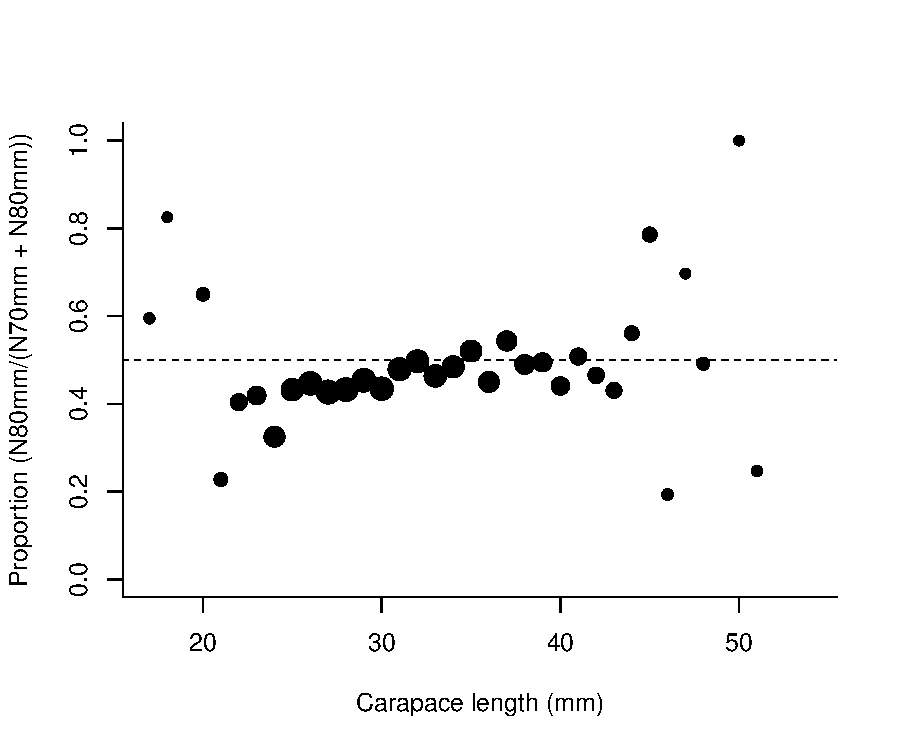
\includegraphics[width=\maxwidth]{figure/rawprops-1} \caption[Proportion of Nephrops raised numbers retained in the 80mm over the sum of the 80mm and 70mm meshes]{Proportion of Nephrops raised numbers retained in the 80mm over the sum of the 80mm and 70mm meshes.}\label{fig:rawprops}
\end{figure}


\end{knitrout}

\section{Models}
A catch comparison binomial Generalized Additive/Linear Mixed Model is suitable choice for these count data where we are interested in estimating how the proportion changes with carapace length. We first try a model with only carapace length as an explanatory variable with haul random effects.

\begin{knitrout}\footnotesize
\definecolor{shadecolor}{rgb}{0.969, 0.969, 0.969}\color{fgcolor}\begin{kframe}
\begin{alltt}
\hlkwd{library}\hlstd{(mgcv)}

\hlstd{neph.7080.cast}\hlopt{$}\hlstd{dum} \hlkwb{<-} \hlnum{1}

\hlcom{## no length effect}
\hlstd{gamm.null} \hlkwb{<-} \hlkwd{gam}\hlstd{(}\hlkwd{cbind}\hlstd{(mesh80mm_Count, mesh70mm_Count)} \hlopt{~} \hlnum{1} \hlopt{+}
                 \hlkwd{s}\hlstd{(fHAUL,} \hlkwc{bs}\hlstd{=}\hlstr{"re"}\hlstd{,} \hlkwc{by} \hlstd{= dum),}
                 \hlkwc{offset} \hlstd{=}
                 \hlkwd{log}\hlstd{(mesh80mm_Overall.Sampling.Ratio} \hlopt{/}
                     \hlstd{mesh70mm_Overall.Sampling.Ratio),}
                 \hlkwc{family} \hlstd{= binomial,}
                 \hlkwc{data} \hlstd{= neph.7080.cast)}

\hlstd{gamm.alt} \hlkwb{<-} \hlkwd{gam}\hlstd{(}\hlkwd{cbind}\hlstd{(mesh80mm_Count, mesh70mm_Count)} \hlopt{~}
                \hlkwd{s}\hlstd{(Carapace.length,} \hlkwc{k} \hlstd{=} \hlnum{5}\hlstd{)} \hlopt{+}
                \hlkwd{s}\hlstd{(fHAUL,} \hlkwc{bs}\hlstd{=}\hlstr{"re"}\hlstd{,} \hlkwc{by} \hlstd{= dum),}
                \hlkwc{offset} \hlstd{=}
                \hlkwd{log}\hlstd{(mesh80mm_Overall.Sampling.Ratio} \hlopt{/}
                    \hlstd{mesh70mm_Overall.Sampling.Ratio),}
                \hlkwc{family} \hlstd{= binomial,}
                \hlkwc{data} \hlstd{= neph.7080.cast)}

\hlcom{## likelihood ratio test for the significance of carapace length}
\hlkwd{anova}\hlstd{(gamm.null, gamm.alt,} \hlkwc{test} \hlstd{=} \hlstr{"Chisq"}\hlstd{)}
\end{alltt}
\begin{verbatim}
## Analysis of Deviance Table
## 
## Model 1: cbind(mesh80mm_Count, mesh70mm_Count) ~ 1 + s(fHAUL, bs = "re", 
##     by = dum)
## Model 2: cbind(mesh80mm_Count, mesh70mm_Count) ~ s(Carapace.length, k = 5) + 
##     s(fHAUL, bs = "re", by = dum)
##   Resid. Df Resid. Dev      Df Deviance Pr(>Chi)   
## 1    324.11     438.09                             
## 2    323.11     429.68 0.99849   8.4149 0.003711 **
## ---
## Signif. codes:  0 '***' 0.001 '**' 0.01 '*' 0.05 '.' 0.1 ' ' 1
\end{verbatim}
\end{kframe}
\end{knitrout}

Plot the predictions from this model.

\begin{knitrout}\footnotesize
\definecolor{shadecolor}{rgb}{0.969, 0.969, 0.969}\color{fgcolor}\begin{kframe}
\begin{alltt}
\hlstd{mean.catch} \hlkwb{<-} \hlkwd{mean}\hlstd{(}\hlkwd{c}\hlstd{(}\hlkwd{unique}\hlstd{(neph.7080.cast}\hlopt{$}\hlstd{mesh70mm_Total.catch),}
                     \hlkwd{unique}\hlstd{(neph.7080.cast}\hlopt{$}\hlstd{mesh80mm_Total.catch)))}

\hlcom{## data frame to predictfor}
\hlstd{pred.df} \hlkwb{<-} \hlkwd{data.frame}\hlstd{(}\hlkwc{Carapace.length} \hlstd{= cl.vec,}
                      \hlkwc{fHAUL} \hlstd{=} \hlstr{"H1"}\hlstd{,}
                      \hlkwc{dum} \hlstd{=} \hlnum{0}\hlstd{,}
                      \hlkwc{mesh80mm_Overall.Sampling.Ratio} \hlstd{=} \hlnum{1}\hlstd{,}
                      \hlkwc{mesh70mm_Overall.Sampling.Ratio} \hlstd{=} \hlnum{1}\hlstd{,}
                      \hlkwc{mesh70mm_Total.catch} \hlstd{= mean.catch,}
                      \hlkwc{mesh80mm_Total.catch} \hlstd{= mean.catch}
                      \hlstd{)}

\hlstd{pred.gamm.alt} \hlkwb{<-} \hlkwd{predict}\hlstd{(gamm.alt,} \hlkwc{newdata} \hlstd{= pred.df,} \hlkwc{se.fit} \hlstd{=} \hlnum{TRUE}\hlstd{)}

\hlcom{## predicted proportions and confidence intervals}
\hlstd{pred.df}\hlopt{$}\hlstd{pred.prop} \hlkwb{<-} \hlkwd{plogis}\hlstd{(pred.gamm.alt}\hlopt{$}\hlstd{fit)}
\hlstd{pred.df}\hlopt{$}\hlstd{lwr.prop} \hlkwb{<-} \hlkwd{plogis}\hlstd{(pred.gamm.alt}\hlopt{$}\hlstd{fit} \hlopt{-} \hlkwd{qnorm}\hlstd{(}\hlnum{0.975}\hlstd{)} \hlopt{*} \hlstd{pred.gamm.alt}\hlopt{$}\hlstd{se.fit)}
\hlstd{pred.df}\hlopt{$}\hlstd{upr.prop} \hlkwb{<-} \hlkwd{plogis}\hlstd{(pred.gamm.alt}\hlopt{$}\hlstd{fit} \hlopt{+} \hlkwd{qnorm}\hlstd{(}\hlnum{0.975}\hlstd{)} \hlopt{*} \hlstd{pred.gamm.alt}\hlopt{$}\hlstd{se.fit)}


\hlkwd{with}\hlstd{(count.df,} \hlkwd{plot}\hlstd{(Carapace.length, prop.80,} \hlkwc{ylim} \hlstd{=} \hlkwd{c}\hlstd{(}\hlnum{0}\hlstd{,} \hlnum{1}\hlstd{),} \hlkwc{pch} \hlstd{=} \hlnum{19}\hlstd{,}
                    \hlkwc{xlab} \hlstd{=} \hlstr{"Carapace length (mm)"}\hlstd{,}
                    \hlkwc{ylab} \hlstd{=} \hlstr{"Proportion (N80mm/(N70mm + N80mm))"}\hlstd{,}
                    \hlkwc{bty} \hlstd{=} \hlstr{"L"}\hlstd{,}
                    \hlkwc{cex} \hlstd{=} \hlnum{1}\hlopt{/}\hlnum{5} \hlopt{*} \hlkwd{log}\hlstd{(N)))}

\hlkwd{with}\hlstd{(pred.df,} \hlkwd{lines}\hlstd{(Carapace.length, pred.prop))}
\hlkwd{with}\hlstd{(pred.df,} \hlkwd{lines}\hlstd{(Carapace.length, lwr.prop,} \hlkwc{lty} \hlstd{=} \hlnum{2}\hlstd{))}
\hlkwd{with}\hlstd{(pred.df,} \hlkwd{lines}\hlstd{(Carapace.length, upr.prop,} \hlkwc{lty} \hlstd{=} \hlnum{2}\hlstd{))}
\hlkwd{abline}\hlstd{(}\hlkwc{h} \hlstd{=} \hlnum{0.5}\hlstd{,} \hlkwc{col} \hlstd{=} \hlstr{"slategrey"}\hlstd{)}
\end{alltt}
\end{kframe}\begin{figure}
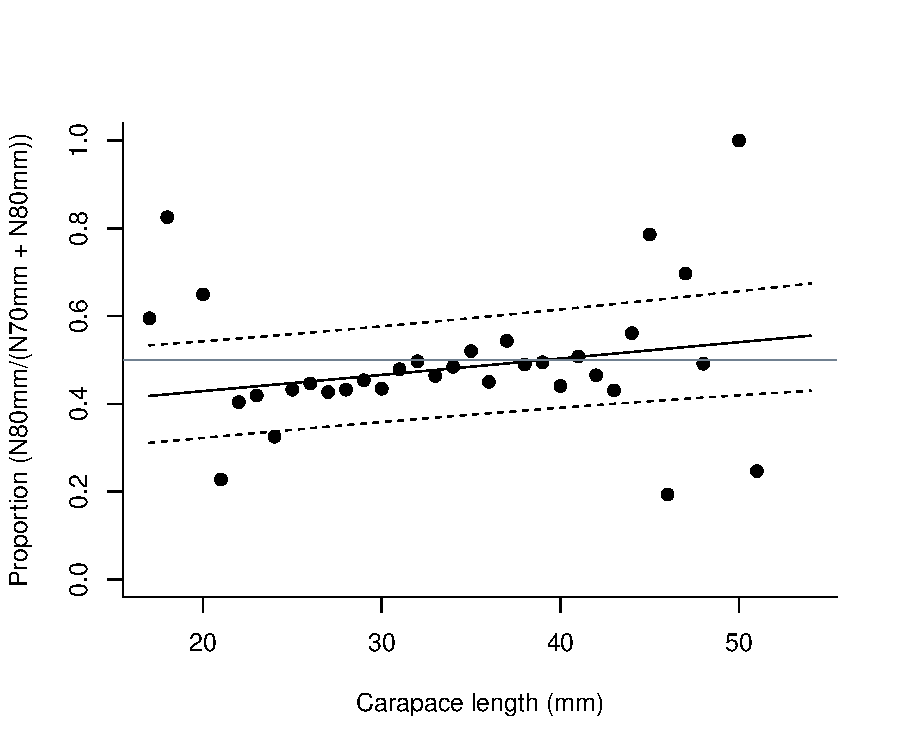
\includegraphics[width=\maxwidth]{figure/glmmsimple-1} \caption[Predicted proportion from binomial GLMM without covariates]{Predicted proportion from binomial GLMM without covariates.}\label{fig:glmmsimple}
\end{figure}


\end{knitrout}

The cause of the wide confidence intervals (Figure ~ \ref{fig:glmmsimple}) is the large amount of inter-haul variability in the proportion retained in the 80mm (Figure~\ref{fig:haulprop})

\begin{knitrout}\footnotesize
\definecolor{shadecolor}{rgb}{0.969, 0.969, 0.969}\color{fgcolor}\begin{kframe}
\begin{alltt}
\hlcom{## Get the proportion at length by haul}
\hlstd{haul.count.df} \hlkwb{<-} \hlkwd{expand.grid}\hlstd{(}\hlkwc{Carapace.length} \hlstd{= cl.vec,}
                             \hlkwc{fHAUL} \hlstd{=} \hlkwd{unique}\hlstd{(neph.7080.cast}\hlopt{$}\hlstd{fHAUL))}

\hlcom{## order the levels}
\hlstd{haul.count.df}\hlopt{$}\hlstd{fHAUL} \hlkwb{<-} \hlkwd{factor}\hlstd{(}\hlkwd{as.character}\hlstd{(haul.count.df}\hlopt{$}\hlstd{fHAUL),}
                              \hlkwc{levels} \hlstd{=} \hlkwd{c}\hlstd{(}\hlkwd{paste}\hlstd{(}\hlstr{"H"}\hlstd{,} \hlnum{1}\hlopt{:}\hlnum{12}\hlstd{,} \hlkwc{sep} \hlstd{=} \hlstr{""}\hlstd{),} \hlstr{"H14"}\hlstd{))}

\hlstd{haul.count.df}\hlopt{$}\hlstd{prop.80} \hlkwb{<-} \hlnum{NA}
\hlstd{haul.count.df}\hlopt{$}\hlstd{N} \hlkwb{<-} \hlnum{NA}
\hlstd{haul.count.df}\hlopt{$}\hlstd{lwr} \hlkwb{<-} \hlnum{NA}
\hlstd{haul.count.df}\hlopt{$}\hlstd{upr} \hlkwb{<-} \hlnum{NA}

\hlkwa{for}\hlstd{(i} \hlkwa{in} \hlnum{1}\hlopt{:}\hlkwd{dim}\hlstd{(haul.count.df)[}\hlnum{1}\hlstd{])\{}
  \hlstd{sub.dat} \hlkwb{<-} \hlkwd{subset}\hlstd{(neph.7080.cast,}
                    \hlstd{Carapace.length} \hlopt{==} \hlstd{haul.count.df}\hlopt{$}\hlstd{Carapace.length[i]} \hlopt{&}
                    \hlstd{fHAUL} \hlopt{==} \hlstd{haul.count.df}\hlopt{$}\hlstd{fHAUL[i])}
  \hlcom{##}
  \hlcom{##if((sub.dat$mesh80mm_Raised.count + sub.dat$mesh70mm_Raised.count) > 0)\{}
  \hlkwa{if}\hlstd{(}\hlkwd{dim}\hlstd{(sub.dat)[}\hlnum{1}\hlstd{]} \hlopt{>} \hlnum{0}\hlstd{)\{}
    \hlstd{btest} \hlkwb{<-} \hlkwd{with}\hlstd{(sub.dat,}
                  \hlkwd{binom.test}\hlstd{(}\hlkwc{x} \hlstd{=} \hlkwd{round}\hlstd{(mesh80mm_Raised.count),}
                             \hlkwc{n} \hlstd{=} \hlkwd{round}\hlstd{(mesh80mm_Raised.count} \hlopt{+} \hlstd{mesh70mm_Raised.count)))}
    \hlcom{##}
    \hlstd{haul.count.df}\hlopt{$}\hlstd{N[i]} \hlkwb{<-} \hlkwd{with}\hlstd{(sub.dat,}
                               \hlkwd{round}\hlstd{(mesh80mm_Raised.count} \hlopt{+} \hlstd{mesh70mm_Raised.count))}
    \hlstd{haul.count.df}\hlopt{$}\hlstd{prop.80[i]} \hlkwb{<-} \hlstd{btest}\hlopt{$}\hlstd{estimate}
    \hlstd{haul.count.df}\hlopt{$}\hlstd{lwr[i]} \hlkwb{<-} \hlstd{btest}\hlopt{$}\hlstd{conf.int[}\hlnum{1}\hlstd{]}
    \hlstd{haul.count.df}\hlopt{$}\hlstd{upr[i]} \hlkwb{<-} \hlstd{btest}\hlopt{$}\hlstd{conf.int[}\hlnum{2}\hlstd{]}
    \hlcom{##}
    \hlkwd{rm}\hlstd{(}\hlkwc{list} \hlstd{=} \hlkwd{c}\hlstd{(}\hlstr{"sub.dat"}\hlstd{,} \hlstr{"btest"}\hlstd{))}
  \hlstd{\}}
\hlstd{\}}

\hlcom{## get predictions at the HAUL level from model}
\hlstd{haul.count.df}\hlopt{$}\hlstd{dum} \hlkwb{<-} \hlnum{1}
\hlstd{haul.count.df}\hlopt{$}\hlstd{pred.prop} \hlkwb{<-} \hlkwd{plogis}\hlstd{(}\hlkwd{predict}\hlstd{(gamm.alt,} \hlkwc{newdata} \hlstd{= haul.count.df))}


\hlkwd{library}\hlstd{(ggplot2)}

\hlstd{blue2red} \hlkwb{<-} \hlkwd{colorRampPalette}\hlstd{(}\hlkwd{c}\hlstd{(}\hlstr{"darkblue"}\hlstd{,} \hlstr{"white"}\hlstd{,} \hlstr{"red"}\hlstd{))}

\hlkwd{ggplot}\hlstd{(haul.count.df,} \hlkwd{aes}\hlstd{(}\hlkwc{x} \hlstd{= Carapace.length,} \hlkwc{y} \hlstd{= prop.80))} \hlopt{+}
  \hlkwd{geom_point}\hlstd{(}\hlkwd{aes}\hlstd{(}\hlkwc{colour} \hlstd{= fHAUL,} \hlkwc{size} \hlstd{=} \hlnum{1}\hlopt{/}\hlnum{5} \hlopt{*} \hlkwd{log}\hlstd{(N)))} \hlopt{+}
  \hlkwd{geom_line}\hlstd{(}\hlkwc{data} \hlstd{= haul.count.df,} \hlkwd{aes}\hlstd{(}\hlkwc{x} \hlstd{= Carapace.length,} \hlkwc{y} \hlstd{= pred.prop,}  \hlkwc{colour} \hlstd{= fHAUL))} \hlopt{+}
  \hlkwd{scale_colour_manual}\hlstd{(}\hlkwc{values} \hlstd{=} \hlkwd{blue2red}\hlstd{(}\hlnum{13}\hlstd{))} \hlopt{+} \hlkwd{ylab}\hlstd{(}\hlstr{"Proportion in 80mm"}\hlstd{)}
\end{alltt}


{\ttfamily\noindent\color{warningcolor}{\#\# Warning: Removed 118 rows containing missing values (geom\_point).}}\end{kframe}\begin{figure}
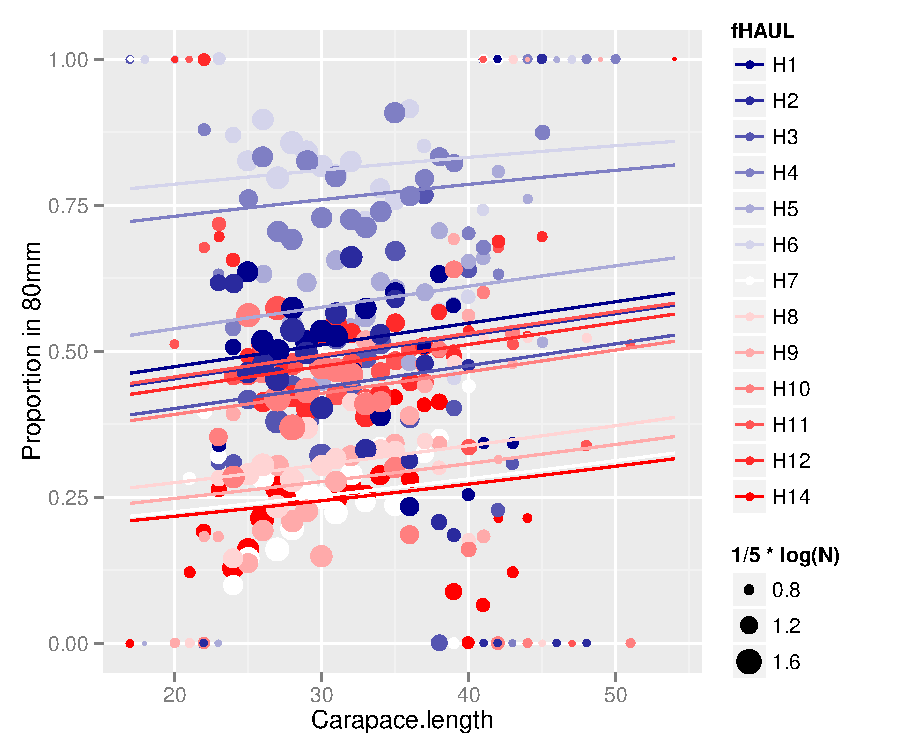
\includegraphics[width=\maxwidth]{figure/haulprop-1} \caption[Observed proportion in the 80mm by haul]{Observed proportion in the 80mm by haul. Note the wide variability of the proportion with some having much higher or lower proportions. Fitted lines come from the GLMM with carapace length only.}\label{fig:haulprop}
\end{figure}


\end{knitrout}

We can take a look at additional measured covariates to see if these relate to the haul-level variability (random effects in the model above) (Figure~\ref{fig:ranefplots}). Firstly, read in the haul duration data

\begin{knitrout}\footnotesize
\definecolor{shadecolor}{rgb}{0.969, 0.969, 0.969}\color{fgcolor}\begin{kframe}
\begin{alltt}
\hlstd{gear.details} \hlkwb{<-} \hlkwd{read.xls}\hlstd{(}\hlstr{"../data/2015 BIM Nephrops quad rig trials/Our Lass 2 70_80_90_100mm codends Irish Sea July 2015/Irish Sea data.xlsx"}\hlstd{,} \hlkwc{sheet} \hlstd{=} \hlnum{2}\hlstd{)}

\hlcom{## merge with the neph data }
\hlstd{gear.details}\hlopt{$}\hlstd{fHAUL} \hlkwb{<-} \hlkwd{factor}\hlstd{(}\hlkwd{paste}\hlstd{(}\hlstr{"H"}\hlstd{, gear.details}\hlopt{$}\hlstd{Tow..,} \hlkwc{sep} \hlstd{=} \hlstr{""}\hlstd{))}

\hlstd{tmp} \hlkwb{<-} \hlkwd{strsplit}\hlstd{(}\hlkwd{as.character}\hlstd{(gear.details}\hlopt{$}\hlstd{Tow.duration),} \hlkwc{split} \hlstd{=} \hlstr{":"}\hlstd{)}

\hlstd{hr} \hlkwb{<-} \hlkwd{as.numeric}\hlstd{(}\hlkwd{unlist}\hlstd{(}\hlkwd{lapply}\hlstd{(tmp,} \hlstr{"["}\hlstd{,} \hlnum{1}\hlstd{)))}
\hlstd{min} \hlkwb{<-} \hlkwd{as.numeric}\hlstd{(}\hlkwd{unlist}\hlstd{(}\hlkwd{lapply}\hlstd{(tmp,} \hlstr{"["}\hlstd{,} \hlnum{2}\hlstd{)))}

\hlstd{gear.details}\hlopt{$}\hlstd{dec.hr} \hlkwb{<-} \hlstd{hr} \hlopt{+} \hlstd{min} \hlopt{/} \hlnum{60}
\end{alltt}
\end{kframe}
\end{knitrout}


\begin{knitrout}\footnotesize
\definecolor{shadecolor}{rgb}{0.969, 0.969, 0.969}\color{fgcolor}\begin{kframe}
\begin{alltt}
\hlcom{##}
\hlstd{ranef.df} \hlkwb{<-} \hlkwd{data.frame}\hlstd{(}\hlkwc{fHAUL} \hlstd{=} \hlkwd{levels}\hlstd{(neph.7080.cast}\hlopt{$}\hlstd{fHAUL),}
                       \hlkwc{ranef} \hlstd{=} \hlkwd{coef}\hlstd{(gamm.alt)[}\hlopt{-}\hlkwd{c}\hlstd{(}\hlnum{1}\hlopt{:}\hlnum{5}\hlstd{)])}
\hlcom{##}
\hlstd{covar.names} \hlkwb{<-} \hlkwd{c}\hlstd{(}\hlstr{"fHAUL"}\hlstd{,} \hlstr{"mesh70mm_Net.position"}\hlstd{,} \hlstr{"mesh70mm_Total.catch"}\hlstd{,}
                 \hlstr{"mesh80mm_Net.position"}\hlstd{,} \hlstr{"mesh80mm_Total.catch"}\hlstd{)}
\hlcom{##}
\hlstd{covar.df} \hlkwb{<-} \hlkwd{unique}\hlstd{(neph.7080.cast[, covar.names])}
\hlcom{## include haul duration}
\hlstd{covar.df} \hlkwb{<-} \hlkwd{merge}\hlstd{(covar.df, gear.details[,} \hlkwd{c}\hlstd{(}\hlstr{"fHAUL"}\hlstd{,} \hlstr{"dec.hr"}\hlstd{)])}
\hlcom{##}
\hlstd{ranef.df} \hlkwb{<-} \hlkwd{merge}\hlstd{(ranef.df, covar.df)}
\hlcom{## convert to long format for plotting}
\hlstd{ranef.df} \hlkwb{<-} \hlkwd{melt}\hlstd{(ranef.df,} \hlkwc{id} \hlstd{=} \hlkwd{c}\hlstd{(}\hlstr{"fHAUL"}\hlstd{,} \hlstr{"ranef"}\hlstd{))}

\hlcom{##}
\hlkwd{ggplot}\hlstd{(ranef.df,} \hlkwd{aes}\hlstd{(}\hlkwc{x} \hlstd{= value,} \hlkwc{y} \hlstd{= ranef))} \hlopt{+}
  \hlkwd{geom_point}\hlstd{()} \hlopt{+}
  \hlkwd{facet_wrap}\hlstd{(}\hlopt{~} \hlstd{variable,} \hlkwc{scales} \hlstd{=} \hlstr{"free"}\hlstd{)} \hlopt{+}
  \hlkwd{xlab}\hlstd{(}\hlstr{"Covariate value"}\hlstd{)} \hlopt{+}
  \hlkwd{ylab}\hlstd{(}\hlstr{"Random effect"}\hlstd{)}
\end{alltt}
\end{kframe}\begin{figure}
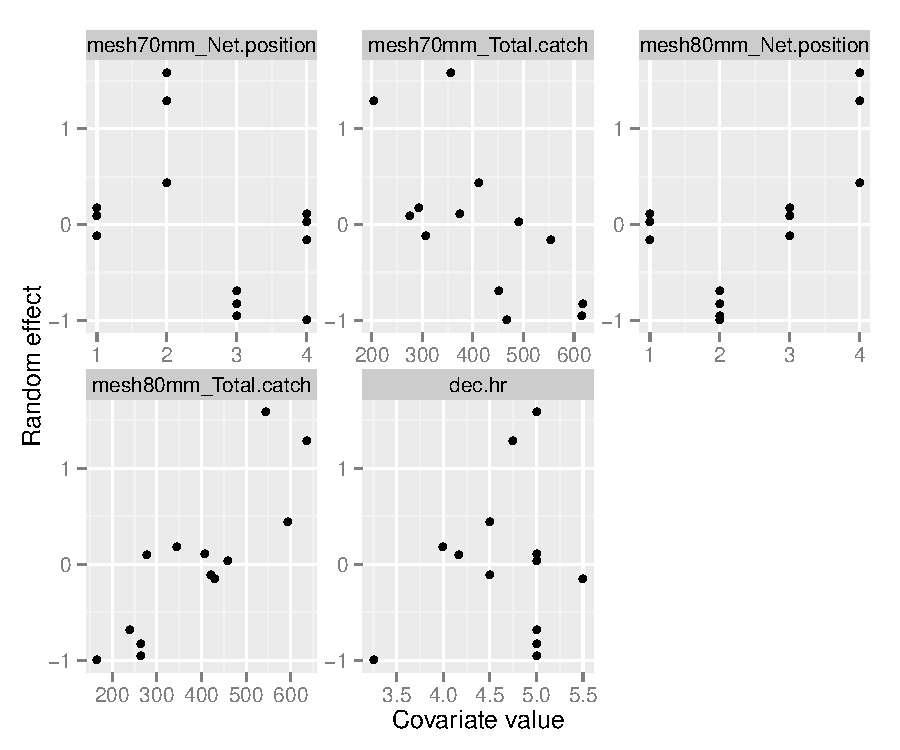
\includegraphics[width=\maxwidth]{figure/ranefplots-1} \caption[Relationship between the random effects of the carapace length only model and measured covariates ]{Relationship between the random effects of the carapace length only model and measured covariates .}\label{fig:ranefplots}
\end{figure}


\end{knitrout}

There are some strong relationships between the random effects and measured covariates (Figure~\ref{fig:ranefplots}). It is best to include these measured variables in the model as fixed effects.

\begin{knitrout}\footnotesize
\definecolor{shadecolor}{rgb}{0.969, 0.969, 0.969}\color{fgcolor}\begin{kframe}
\begin{alltt}
\hlkwd{library}\hlstd{(lme4)}
\hlkwd{library}\hlstd{(effects)}

\hlcom{## including additional covariates}
\hlcom{## check identifiability}
\hlstd{neph.7080.cast}\hlopt{$}\hlstd{fmesh80mm_Net.position} \hlkwb{<-}
  \hlkwd{factor}\hlstd{(}\hlkwd{paste}\hlstd{(}\hlstr{"pos"}\hlstd{,}
               \hlstd{neph.7080.cast}\hlopt{$}\hlstd{mesh80mm_Net.position,} \hlkwc{sep} \hlstd{=} \hlstr{""}\hlstd{))}

\hlstd{neph.7080.cast} \hlkwb{<-} \hlkwd{merge}\hlstd{(neph.7080.cast, gear.details[,} \hlkwd{c}\hlstd{(}\hlstr{"fHAUL"}\hlstd{,} \hlstr{"dec.hr"}\hlstd{)])}

\hlcom{## using log of total catch weights - return to this}
\hlstd{neph.7080.cast}\hlopt{$}\hlstd{log.mesh80mm_Total.catch} \hlkwb{<-} \hlkwd{log}\hlstd{(neph.7080.cast}\hlopt{$}\hlstd{mesh80mm_Total.catch)}
\hlstd{neph.7080.cast}\hlopt{$}\hlstd{log.mesh70mm_Total.catch} \hlkwb{<-} \hlkwd{log}\hlstd{(neph.7080.cast}\hlopt{$}\hlstd{mesh70mm_Total.catch)}

\hlstd{max.Carapace.length} \hlkwb{<-} \hlkwd{max}\hlstd{(neph.7080.cast}\hlopt{$}\hlstd{Carapace.length)}
\hlstd{neph.7080.cast}\hlopt{$}\hlstd{prop.Carapace.length} \hlkwb{<-} \hlstd{neph.7080.cast}\hlopt{$}\hlstd{Carapace.length} \hlopt{/} \hlstd{max.Carapace.length}

\hlcom{## Note should return to this warning later}
\hlcom{## fits okay in gam but glmm used for effects package}
\hlstd{glmm.alt.covar} \hlkwb{<-} \hlkwd{glmer}\hlstd{(}\hlkwd{cbind}\hlstd{(mesh80mm_Count, mesh70mm_Count)} \hlopt{~}
                        \hlcom{##I(log(mesh80mm_Total.catch / mesh70mm_Total.catch)) * Carapace.length +}
                        \hlstd{log.mesh80mm_Total.catch} \hlopt{+} \hlstd{log.mesh70mm_Total.catch} \hlopt{+}
                        \hlstd{prop.Carapace.length} \hlopt{+}
                        \hlstd{fmesh80mm_Net.position} \hlopt{+}
                        \hlstd{(}\hlnum{1} \hlopt{|} \hlstd{fHAUL),}
                        \hlkwc{offset} \hlstd{=}
                        \hlkwd{log}\hlstd{(mesh80mm_Overall.Sampling.Ratio} \hlopt{/}
                            \hlstd{mesh70mm_Overall.Sampling.Ratio),}
                        \hlkwc{family} \hlstd{= binomial,}
                        \hlkwc{data} \hlstd{= neph.7080.cast,}
                        \hlkwc{control}\hlstd{=}\hlkwd{glmerControl}\hlstd{(}\hlkwc{optimizer}\hlstd{=}\hlstr{"bobyqa"}\hlstd{))}

\hlstd{glmm.alt.covar.catchdur} \hlkwb{<-} \hlkwd{glmer}\hlstd{(}\hlkwd{cbind}\hlstd{(mesh80mm_Count, mesh70mm_Count)} \hlopt{~}
                                 \hlcom{##I(log(mesh80mm_Total.catch / mesh70mm_Total.catch)) * Carapace.length +}
                                 \hlstd{log.mesh80mm_Total.catch} \hlopt{+} \hlstd{log.mesh70mm_Total.catch} \hlopt{+}
                                 \hlstd{prop.Carapace.length} \hlopt{+}
                                 \hlstd{fmesh80mm_Net.position} \hlopt{+}
                                 \hlkwd{poly}\hlstd{(dec.hr,} \hlnum{1}\hlstd{)} \hlopt{+}
                                 \hlstd{(}\hlnum{1} \hlopt{|} \hlstd{fHAUL),}
                                 \hlkwc{offset} \hlstd{=}
                                 \hlkwd{log}\hlstd{(mesh80mm_Overall.Sampling.Ratio} \hlopt{/}
                                     \hlstd{mesh70mm_Overall.Sampling.Ratio),}
                                 \hlkwc{family} \hlstd{= binomial,}
                                 \hlkwc{data} \hlstd{= neph.7080.cast,}
                                 \hlkwc{control}\hlstd{=}\hlkwd{glmerControl}\hlstd{(}\hlkwc{optimizer}\hlstd{=}\hlstr{"bobyqa"}\hlstd{))}

\hlstd{glmm.alt.covar.catchdur.nobulk} \hlkwb{<-} \hlkwd{glmer}\hlstd{(}\hlkwd{cbind}\hlstd{(mesh80mm_Count, mesh70mm_Count)} \hlopt{~}
                                        \hlcom{##I(log(mesh80mm_Total.catch / mesh70mm_Total.catch)) * Carapace.length +}
                                        \hlcom{##log.mesh80mm_Total.catch + log.mesh70mm_Total.catch + }
                                        \hlstd{prop.Carapace.length} \hlopt{+}
                                        \hlstd{fmesh80mm_Net.position} \hlopt{+}
                                        \hlkwd{poly}\hlstd{(dec.hr,} \hlnum{1}\hlstd{)} \hlopt{+}
                                        \hlstd{(}\hlnum{1} \hlopt{|} \hlstd{fHAUL),}
                                        \hlkwc{offset} \hlstd{=}
                                        \hlkwd{log}\hlstd{(mesh80mm_Overall.Sampling.Ratio} \hlopt{/}
                                            \hlstd{mesh70mm_Overall.Sampling.Ratio),}
                                        \hlkwc{family} \hlstd{= binomial,}
                                        \hlkwc{data} \hlstd{= neph.7080.cast,}
                                        \hlkwc{control}\hlstd{=}\hlkwd{glmerControl}\hlstd{(}\hlkwc{optimizer}\hlstd{=}\hlstr{"bobyqa"}\hlstd{))}

\hlcom{## include squared length term}
\hlstd{glmm.alt.covar2} \hlkwb{<-} \hlkwd{glmer}\hlstd{(}\hlkwd{cbind}\hlstd{(mesh80mm_Count, mesh70mm_Count)} \hlopt{~}
                         \hlcom{##I(log(mesh80mm_Total.catch / mesh70mm_Total.catch)) * Carapace.length +}
                         \hlstd{log.mesh80mm_Total.catch} \hlopt{+} \hlstd{log.mesh70mm_Total.catch} \hlopt{+}
                         \hlkwd{poly}\hlstd{(prop.Carapace.length,} \hlnum{2}\hlstd{)} \hlopt{+}
                         \hlkwd{poly}\hlstd{(dec.hr,} \hlnum{1}\hlstd{)} \hlopt{+}
                         \hlstd{fmesh80mm_Net.position} \hlopt{+}
                         \hlstd{(}\hlnum{1} \hlopt{|} \hlstd{fHAUL),}
                         \hlkwc{offset} \hlstd{=}
                         \hlkwd{log}\hlstd{(mesh80mm_Overall.Sampling.Ratio} \hlopt{/}
                             \hlstd{mesh70mm_Overall.Sampling.Ratio),}
                         \hlkwc{family} \hlstd{= binomial,}
                         \hlkwc{data} \hlstd{= neph.7080.cast,}
                         \hlkwc{control}\hlstd{=}\hlkwd{glmerControl}\hlstd{(}\hlkwc{optimizer}\hlstd{=}\hlstr{"bobyqa"}\hlstd{))}

\hlcom{## in GAM}
\hlstd{gamm.alt.covar2} \hlkwb{<-} \hlkwd{gam}\hlstd{(}\hlkwd{cbind}\hlstd{(mesh80mm_Count, mesh70mm_Count)} \hlopt{~}
                       \hlcom{##I(log(mesh80mm_Total.catch / mesh70mm_Total.catch)) * Carapace.length +}
                       \hlstd{log.mesh80mm_Total.catch} \hlopt{+} \hlstd{log.mesh70mm_Total.catch} \hlopt{+}
                       \hlkwd{s}\hlstd{(prop.Carapace.length,} \hlkwc{k} \hlstd{=} \hlnum{5}\hlstd{,} \hlkwc{fx} \hlstd{=} \hlnum{TRUE}\hlstd{)} \hlopt{+}
                       \hlkwd{poly}\hlstd{(dec.hr,} \hlnum{1}\hlstd{)} \hlopt{+}
                       \hlstd{fmesh80mm_Net.position} \hlopt{+}
                       \hlkwd{s}\hlstd{(fHAUL,} \hlkwc{bs}\hlstd{=}\hlstr{"re"}\hlstd{,} \hlkwc{by} \hlstd{= dum),}
                       \hlkwc{offset} \hlstd{=}
                       \hlkwd{log}\hlstd{(mesh80mm_Overall.Sampling.Ratio} \hlopt{/}
                           \hlstd{mesh70mm_Overall.Sampling.Ratio),}
                       \hlkwc{family} \hlstd{= binomial,}
                       \hlkwc{data} \hlstd{= neph.7080.cast)}

\hlcom{## use effects package to get prediction for model with net position}
\hlcom{## set predictor variables}
\hlstd{xlevels} \hlkwb{<-} \hlkwd{list}\hlstd{(}\hlkwc{prop.Carapace.length} \hlstd{= cl.vec}\hlopt{/}\hlstd{max.Carapace.length)}

\hlcom{## if we wanted to set the proportions of net positions equivalent}
\hlcom{## otherwise set to the proportion observed in the data}
\hlcom{##given.values <- c("fmesh80mm_Net.positionpos2" = 1/4,}
\hlcom{##                  "fmesh80mm_Net.positionpos3" = 1/4,}
\hlcom{##                  "fmesh80mm_Net.positionpos4" = 1/4}
\hlcom{##                  )}

\hlcom{##cl.effect <- effect("Carapace.length", glmm.alt.covar, xlevels = xlevels, offset = 0, given.values = given.values)}
\hlstd{cl.effect} \hlkwb{<-} \hlkwd{effect}\hlstd{(}\hlstr{"prop.Carapace.length"}\hlstd{, glmm.alt.covar.catchdur,} \hlkwc{xlevels} \hlstd{= xlevels,} \hlkwc{offset} \hlstd{=} \hlnum{0}\hlstd{)}
\end{alltt}
\end{kframe}
\end{knitrout}

Plot the effect of carapace length with the other variables set to their mean in the data (Figure~\ref{fig:glmmcovar}).

\begin{knitrout}\footnotesize
\definecolor{shadecolor}{rgb}{0.969, 0.969, 0.969}\color{fgcolor}\begin{kframe}
\begin{alltt}
\hlkwd{with}\hlstd{(count.df,} \hlkwd{plot}\hlstd{(Carapace.length, prop.80,} \hlkwc{ylim} \hlstd{=} \hlkwd{c}\hlstd{(}\hlnum{0}\hlstd{,} \hlnum{1}\hlstd{),} \hlkwc{pch} \hlstd{=} \hlnum{19}\hlstd{,}
                    \hlkwc{xlab} \hlstd{=} \hlstr{"Carapace length (mm)"}\hlstd{,}
                    \hlkwc{ylab} \hlstd{=} \hlstr{"Proportion (N80mm/(N70mm + N80mm))"}\hlstd{,}
                    \hlkwc{bty} \hlstd{=} \hlstr{"L"}\hlstd{,}
                    \hlkwc{cex} \hlstd{=} \hlnum{1}\hlopt{/}\hlnum{5} \hlopt{*} \hlkwd{log}\hlstd{(N)))}

\hlcom{## effects prediction}
\hlkwd{lines}\hlstd{(cl.vec,} \hlkwd{plogis}\hlstd{(cl.effect}\hlopt{$}\hlstd{fit[,} \hlnum{1}\hlstd{]))}
\hlkwd{lines}\hlstd{(cl.vec,} \hlkwd{plogis}\hlstd{(cl.effect}\hlopt{$}\hlstd{lower[,} \hlnum{1}\hlstd{]),} \hlkwc{lty} \hlstd{=} \hlnum{2}\hlstd{)}
\hlkwd{lines}\hlstd{(cl.vec,} \hlkwd{plogis}\hlstd{(cl.effect}\hlopt{$}\hlstd{upper[,} \hlnum{1}\hlstd{]),} \hlkwc{lty} \hlstd{=} \hlnum{2}\hlstd{)}
\hlkwd{abline}\hlstd{(}\hlkwc{h} \hlstd{=} \hlnum{0.5}\hlstd{,} \hlkwc{col} \hlstd{=} \hlstr{"slategrey"}\hlstd{)}
\end{alltt}
\end{kframe}\begin{figure}
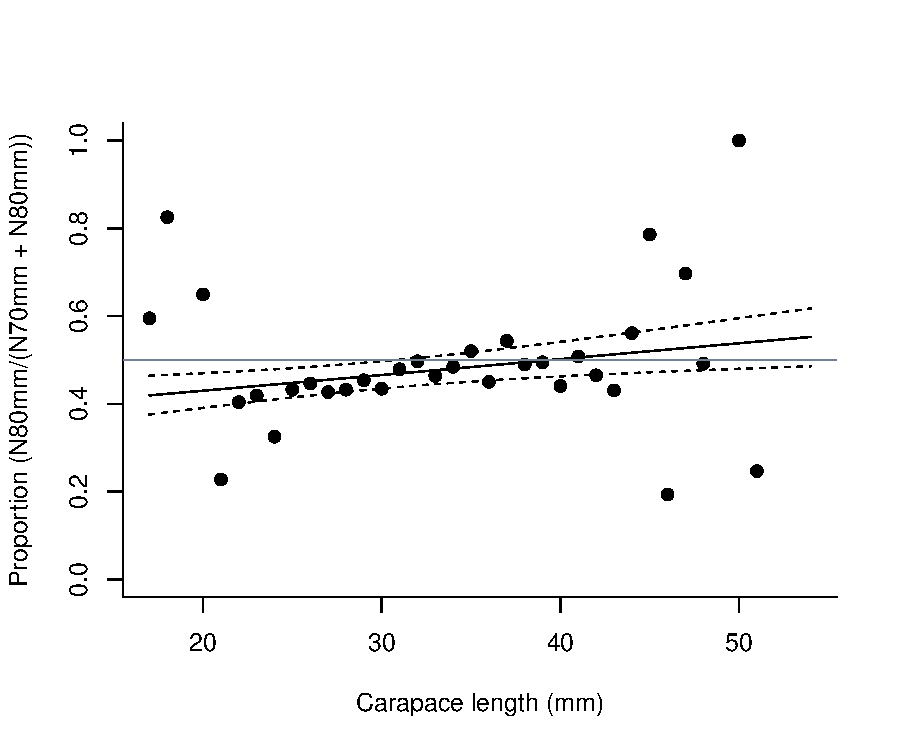
\includegraphics[width=\maxwidth]{figure/glmmcovar-1} \caption[Predicted proportion from binomial GLMM with covariates]{Predicted proportion from binomial GLMM with covariates. Note in the predictions the bulk weights are set to their mean and the net positions to their proportional occurence in the data.}\label{fig:glmmcovar}
\end{figure}

\begin{kframe}\begin{alltt}
\hlcom{## Note the wide confidence intervals}
\end{alltt}
\end{kframe}
\end{knitrout}

Finally test length effect in covariate model
\begin{knitrout}\footnotesize
\definecolor{shadecolor}{rgb}{0.969, 0.969, 0.969}\color{fgcolor}\begin{kframe}
\begin{alltt}
\hlstd{glmm.alt.covar.catchdur.nolength} \hlkwb{<-} \hlkwd{glmer}\hlstd{(}\hlkwd{cbind}\hlstd{(mesh80mm_Count, mesh70mm_Count)} \hlopt{~}
                                          \hlstd{log.mesh80mm_Total.catch} \hlopt{+} \hlstd{log.mesh70mm_Total.catch} \hlopt{+}
                                          \hlstd{fmesh80mm_Net.position} \hlopt{+}
                                          \hlkwd{poly}\hlstd{(dec.hr,} \hlnum{1}\hlstd{)} \hlopt{+}
                                          \hlstd{(}\hlnum{1} \hlopt{|} \hlstd{fHAUL),}
                                          \hlkwc{offset} \hlstd{=}
                                          \hlkwd{log}\hlstd{(mesh80mm_Overall.Sampling.Ratio} \hlopt{/}
                                              \hlstd{mesh70mm_Overall.Sampling.Ratio),}
                                          \hlkwc{family} \hlstd{= binomial,}
                                          \hlkwc{data} \hlstd{= neph.7080.cast,}
                                          \hlkwc{control}\hlstd{=}\hlkwd{glmerControl}\hlstd{(}\hlkwc{optimizer}\hlstd{=}\hlstr{"bobyqa"}\hlstd{))}
\end{alltt}


{\ttfamily\noindent\color{warningcolor}{\#\# Warning in checkConv(attr(opt, "{}derivs"{}), opt\$par, ctrl = control\$checkConv, : Model failed to converge with max|grad| = 0.0073401 (tol = 0.001, component 2)}}\begin{alltt}
\hlcom{## likelihood ratio test}
\hlkwd{anova}\hlstd{(glmm.alt.covar.catchdur.nolength, glmm.alt.covar.catchdur)}
\end{alltt}
\begin{verbatim}
## Data: neph.7080.cast
## Models:
## glmm.alt.covar.catchdur.nolength: cbind(mesh80mm_Count, mesh70mm_Count) ~ log.mesh80mm_Total.catch + 
## glmm.alt.covar.catchdur.nolength:     log.mesh70mm_Total.catch + fmesh80mm_Net.position + poly(dec.hr, 
## glmm.alt.covar.catchdur.nolength:     1) + (1 | fHAUL)
## glmm.alt.covar.catchdur: cbind(mesh80mm_Count, mesh70mm_Count) ~ log.mesh80mm_Total.catch + 
## glmm.alt.covar.catchdur:     log.mesh70mm_Total.catch + prop.Carapace.length + fmesh80mm_Net.position + 
## glmm.alt.covar.catchdur:     poly(dec.hr, 1) + (1 | fHAUL)
##                                  Df    AIC    BIC  logLik deviance  Chisq
## glmm.alt.covar.catchdur.nolength  8 1417.9 1448.5 -700.97   1401.9       
## glmm.alt.covar.catchdur           9 1411.6 1446.0 -696.79   1393.6 8.3654
##                                  Chi Df Pr(>Chisq)   
## glmm.alt.covar.catchdur.nolength                     
## glmm.alt.covar.catchdur               1   0.003824 **
## ---
## Signif. codes:  0 '***' 0.001 '**' 0.01 '*' 0.05 '.' 0.1 ' ' 1
\end{verbatim}
\begin{alltt}
\hlcom{## significant effect of carapace length}
\end{alltt}
\end{kframe}
\end{knitrout}

\section{Economic section}

\begin{knitrout}\footnotesize
\definecolor{shadecolor}{rgb}{0.969, 0.969, 0.969}\color{fgcolor}\begin{kframe}
\begin{alltt}
\hlkwd{curve}\hlstd{(}\hlnum{0.00032} \hlopt{*} \hlstd{x}\hlopt{^}\hlnum{3.21}\hlstd{,} \hlkwc{from} \hlstd{=} \hlnum{0}\hlstd{,} \hlkwc{to} \hlstd{=} \hlnum{60}\hlstd{,} \hlkwc{xlab} \hlstd{=} \hlstr{"Carapace length (mm)"}\hlstd{,}
      \hlkwc{ylab} \hlstd{=} \hlstr{"Total weight (g)"}\hlstd{)}

\hlstd{npkilo.breaks} \hlkwb{<-} \hlkwd{c}\hlstd{(}\hlnum{1}\hlstd{,} \hlnum{11}\hlstd{,} \hlnum{16}\hlstd{,} \hlnum{21}\hlstd{,} \hlnum{31}\hlstd{,} \hlnum{41}\hlstd{,} \hlnum{50}\hlstd{)}
\hlstd{wt.breaks} \hlkwb{<-} \hlstd{(}\hlnum{1}\hlopt{/} \hlstd{npkilo.breaks)} \hlopt{*} \hlnum{1e3}
\hlkwd{abline}\hlstd{(}\hlkwc{h} \hlstd{= wt.breaks,} \hlkwc{col} \hlstd{=} \hlstr{"grey"}\hlstd{)}

\hlcom{## corresponding length cut-offs}
\hlstd{lt.breaks} \hlkwb{=} \hlkwd{exp}\hlstd{(}\hlkwd{log}\hlstd{(wt.breaks} \hlopt{/} \hlnum{0.00032}\hlstd{)}\hlopt{/}\hlnum{3.21}\hlstd{)}
\hlkwd{abline}\hlstd{(}\hlkwc{v} \hlstd{= lt.breaks,} \hlkwc{col} \hlstd{=} \hlstr{"grey"}\hlstd{)}

\hlcom{## below MCRS band}
\hlkwd{abline}\hlstd{(}\hlkwc{v} \hlstd{=} \hlnum{20}\hlstd{)}
\hlkwd{abline}\hlstd{(}\hlkwc{h} \hlstd{=} \hlnum{0.00032}\hlopt{*}\hlnum{20}\hlopt{^}\hlnum{3.21}\hlstd{)}
\end{alltt}
\end{kframe}\begin{figure}
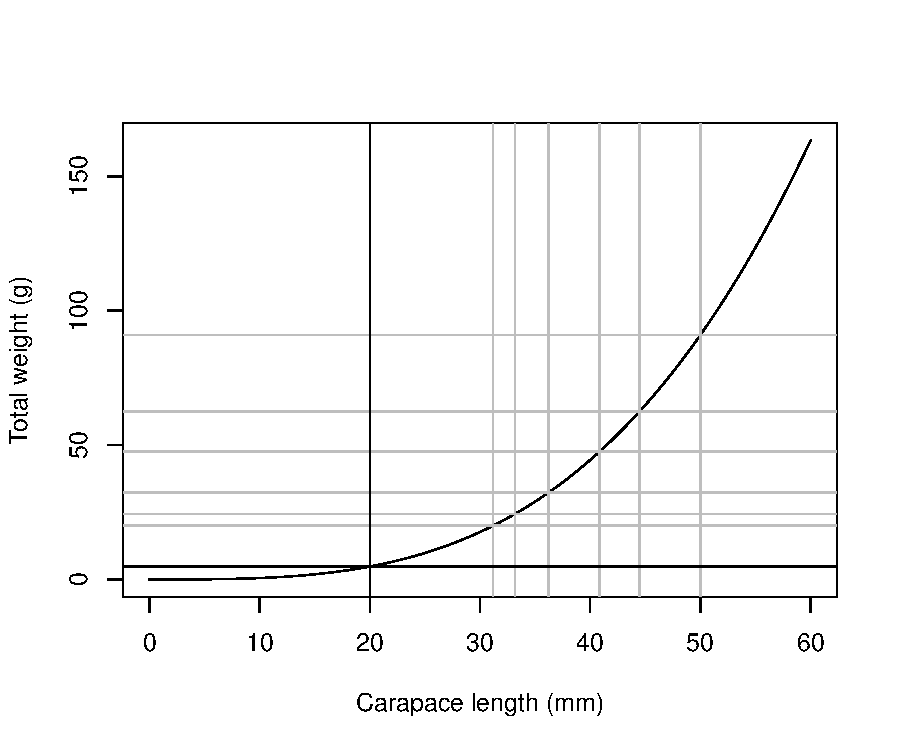
\includegraphics[width=\maxwidth]{figure/lw-1} \caption[Length - weight relationship with horizontal price bands converted to length-based price bands]{Length - weight relationship with horizontal price bands converted to length-based price bands. Price band in black denotes below Minimum Conservation Reference Size prawns.}\label{fig:lw}
\end{figure}


\end{knitrout}

Simulate distributions of retained catches with different means

\begin{knitrout}\footnotesize
\definecolor{shadecolor}{rgb}{0.969, 0.969, 0.969}\color{fgcolor}\begin{kframe}
\begin{alltt}
\hlstd{sim.means} \hlkwb{<-} \hlkwd{c}\hlstd{(}\hlnum{24}\hlstd{,} \hlnum{27}\hlstd{,} \hlnum{33}\hlstd{)}

\hlcom{## get the vector of raised counts for the whole Our Lass trip}
\hlstd{neph.lengths} \hlkwb{<-} \hlkwd{with}\hlstd{(}\hlkwd{subset}\hlstd{(neph.dat, Mesh.Size}\hlopt\hlkwd{c}\hlstd{(}\hlstr{"70mm"}\hlstd{,} \hlstr{"80mm"}\hlstd{)),}
                     \hlkwd{rep}\hlstd{(Carapace.length,} \hlkwc{times} \hlstd{=} \hlkwd{round}\hlstd{(Raised.count.)))}

\hlkwd{length}\hlstd{(neph.lengths)} \hlcom{## raised number of prawns caught}
\end{alltt}
\begin{verbatim}
## [1] 206009
\end{verbatim}
\begin{alltt}
\hlstd{(mean.cl} \hlkwb{<-} \hlkwd{mean}\hlstd{(neph.lengths))} \hlcom{## mean carapace length below}
\end{alltt}
\begin{verbatim}
## [1] 30.09305
\end{verbatim}
\begin{alltt}
\hlcom{## differences in the mean observed length and simulated means}
\hlcom{## plus 0.5 to account for nearest mm below}
\hlstd{sim.diff} \hlkwb{<-} \hlstd{mean.cl} \hlopt{-} \hlstd{(sim.means} \hlopt{+} \hlnum{0.5}\hlstd{)}
\end{alltt}
\end{kframe}
\end{knitrout}

\begin{knitrout}\footnotesize
\definecolor{shadecolor}{rgb}{0.969, 0.969, 0.969}\color{fgcolor}\begin{kframe}
\begin{alltt}
\hlcom{## plot the simulated distributions of retained catches}
\hlstd{hist.orig} \hlkwb{<-} \hlkwd{hist}\hlstd{(neph.lengths,} \hlkwc{breaks} \hlstd{=} \hlkwd{seq}\hlstd{(}\hlnum{0.5}\hlstd{,} \hlnum{60}\hlstd{,} \hlkwc{by} \hlstd{=} \hlnum{1}\hlstd{),} \hlkwc{plot} \hlstd{=} \hlnum{FALSE}\hlstd{)}
\hlcom{##hist.orig <- hist(neph.lengths, breaks = seq(1, 60, by = 1), plot = FALSE)}
\hlstd{cl.mids} \hlkwb{<-} \hlstd{hist.orig}\hlopt{$}\hlstd{mids}
\hlstd{count.sim} \hlkwb{<-} \hlkwd{matrix}\hlstd{(hist.orig}\hlopt{$}\hlstd{counts,} \hlkwc{nrow} \hlstd{=} \hlnum{1}\hlstd{)}

\hlkwd{plot}\hlstd{(hist.orig}\hlopt{$}\hlstd{mids, hist.orig}\hlopt{$}\hlstd{counts,} \hlkwc{type} \hlstd{=} \hlstr{"l"}\hlstd{,} \hlkwc{xlim} \hlstd{=} \hlkwd{c}\hlstd{(}\hlnum{10}\hlstd{,} \hlnum{50}\hlstd{),}
     \hlkwc{xlab} \hlstd{=} \hlstr{"Carapace length (mm)"}\hlstd{,} \hlkwc{ylab} \hlstd{=} \hlstr{"Count per 1 mm bin"}\hlstd{)}
\hlcom{##}
\hlkwa{for}\hlstd{(i} \hlkwa{in} \hlnum{1}\hlopt{:}\hlkwd{length}\hlstd{(sim.means))\{}
  \hlstd{hist.sim} \hlkwb{<-} \hlkwd{hist}\hlstd{(neph.lengths} \hlopt{-} \hlstd{sim.diff[i],}
                   \hlkwc{breaks} \hlstd{=} \hlkwd{seq}\hlstd{(}\hlnum{0.5}\hlstd{,} \hlnum{60}\hlstd{,} \hlkwc{by} \hlstd{=} \hlnum{1}\hlstd{),} \hlkwc{plot} \hlstd{=} \hlnum{FALSE}\hlstd{)}
                   \hlcom{##breaks = seq(1, 60, by = 1), plot = FALSE)}
  \hlkwd{lines}\hlstd{(hist.sim}\hlopt{$}\hlstd{mids, hist.sim}\hlopt{$}\hlstd{counts,} \hlkwc{lty} \hlstd{=} \hlnum{1} \hlopt{+} \hlstd{i,} \hlkwc{col} \hlstd{=} \hlnum{1}\hlopt{+}\hlstd{i)}
  \hlstd{count.sim} \hlkwb{<-} \hlkwd{rbind}\hlstd{(count.sim, hist.sim}\hlopt{$}\hlstd{counts)}
\hlstd{\}}

\hlkwd{legend}\hlstd{(}\hlstr{"topright"}\hlstd{,} \hlkwc{legend} \hlstd{=}
       \hlkwd{c}\hlstd{(}\hlstr{"Original (30.09mm)"}\hlstd{,} \hlstr{"24mm mean"}\hlstd{,}
         \hlstr{"27mm mean"}\hlstd{,} \hlstr{"33mm mean"}\hlstd{),}
       \hlkwc{lty} \hlstd{=} \hlkwd{c}\hlstd{(}\hlnum{1}\hlopt{:}\hlnum{4}\hlstd{),} \hlkwc{col} \hlstd{=} \hlnum{1}\hlopt{:}\hlnum{4}\hlstd{,} \hlkwc{bty} \hlstd{=} \hlstr{"n"}\hlstd{)}
\end{alltt}
\end{kframe}\begin{figure}
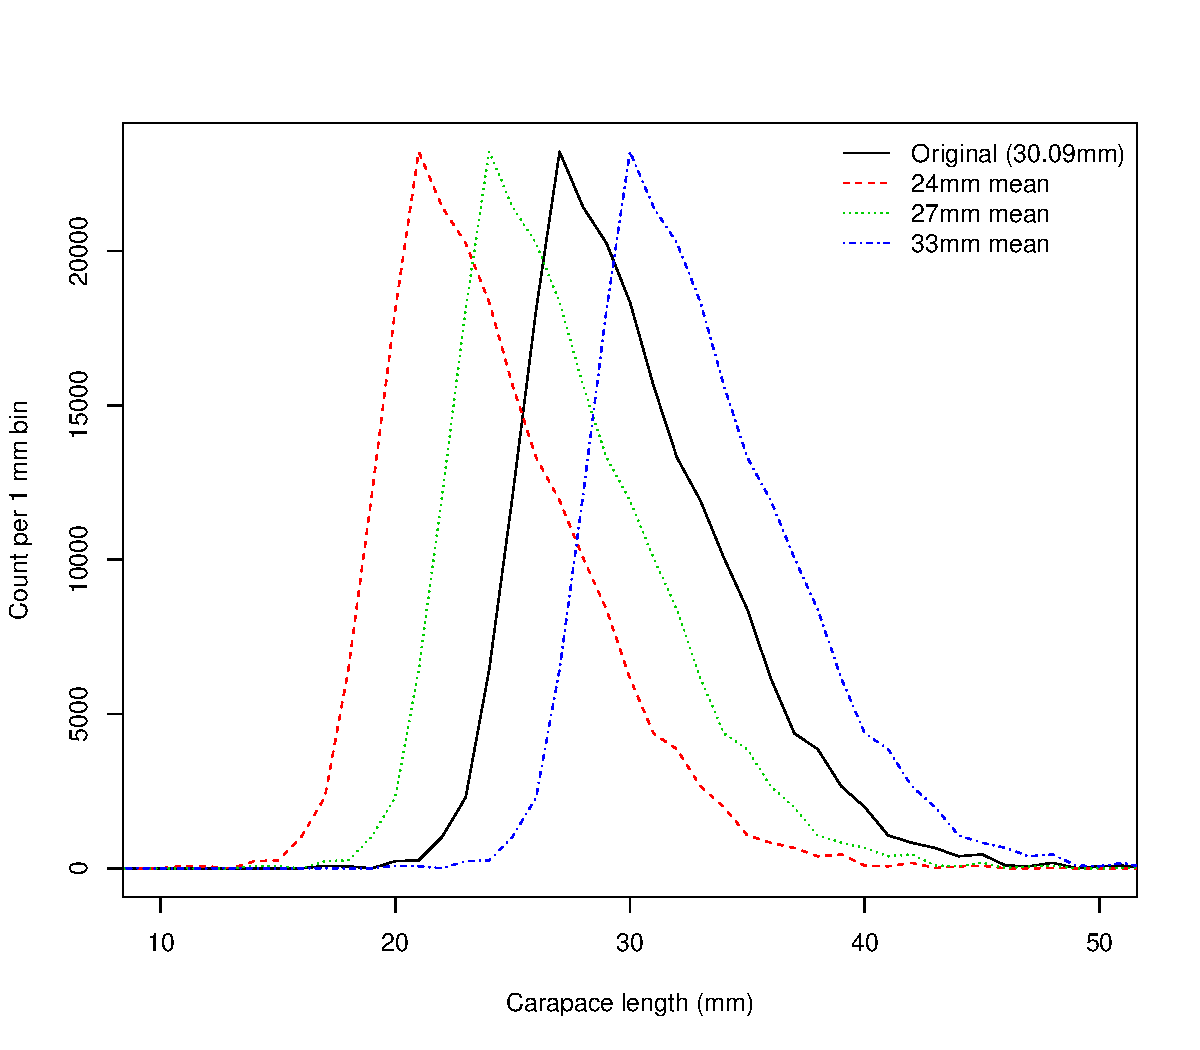
\includegraphics[width=\maxwidth]{figure/simdist-1} \caption[Simulated distributions of retained catches]{Simulated distributions of retained catches.}\label{fig:simdist}
\end{figure}

\begin{kframe}\begin{alltt}
\hlcom{## }
\hlkwd{rownames}\hlstd{(count.sim)} \hlkwb{<-} \hlkwd{c}\hlstd{(}\hlstr{"original"}\hlstd{,} \hlstr{"mm.24"}\hlstd{,} \hlstr{"mm.27"}\hlstd{,} \hlstr{"mm.33"}\hlstd{)}
\end{alltt}
\end{kframe}
\end{knitrout}

Per-haul variables
\begin{knitrout}\footnotesize
\definecolor{shadecolor}{rgb}{0.969, 0.969, 0.969}\color{fgcolor}\begin{kframe}
\begin{alltt}
\hlcom{## count per haul (13 hauls)}
\hlstd{count.phaul.sim} \hlkwb{<-} \hlstd{count.sim} \hlopt{/} \hlstd{(}\hlnum{13}\hlstd{)} \hlcom{## note this is the sum for the 70 and 80}

\hlcom{## get predicted prawn weight per length bin in kgs}
\hlstd{wt.mids} \hlkwb{<-} \hlstd{(}\hlnum{0.00032} \hlopt{*} \hlstd{cl.mids}\hlopt{^}\hlnum{3.21}\hlstd{)} \hlopt{/} \hlnum{1e3}

\hlcom{## get total weight per haul}
\hlstd{wt.phaul.sim} \hlkwb{<-} \hlkwd{t}\hlstd{(}\hlkwd{apply}\hlstd{(count.phaul.sim,} \hlnum{1}\hlstd{,} \hlkwc{FUN} \hlstd{=} \hlkwa{function}\hlstd{(}\hlkwc{z}\hlstd{)\{z} \hlopt{*} \hlstd{wt.mids\}))}

\hlcom{## predicted price per length class }
\hlcom{## note 20mm CL included here}
\hlstd{wt.cuts} \hlkwb{<-} \hlkwd{cut}\hlstd{(wt.mids,} \hlkwc{breaks} \hlstd{=} \hlkwd{c}\hlstd{(wt.breaks,} \hlnum{0.00032}\hlopt{*}\hlnum{20}\hlopt{^}\hlnum{3.21}\hlstd{,} \hlnum{0}\hlstd{)} \hlopt{/} \hlnum{1e3}\hlstd{)}

\hlstd{price.df} \hlkwb{<-}  \hlkwd{data.frame}\hlstd{(}\hlkwc{wt.bin} \hlstd{=} \hlkwd{unique}\hlstd{(wt.cuts),}
                        \hlkwc{price} \hlstd{=} \hlkwd{c}\hlstd{(}\hlopt{-}\hlnum{0.2}\hlstd{,} \hlnum{1.90}\hlstd{,} \hlnum{4.75}\hlstd{,} \hlnum{5.35}\hlstd{,} \hlnum{7.75}\hlstd{,} \hlnum{10.75}\hlstd{,} \hlnum{13}\hlstd{,} \hlnum{13}\hlstd{))}

\hlstd{price.df}
\end{alltt}
\begin{verbatim}
##            wt.bin price
## 1      (0,0.0048] -0.20
## 2   (0.0048,0.02]  1.90
## 3   (0.02,0.0244]  4.75
## 4 (0.0244,0.0323]  5.35
## 5 (0.0323,0.0476]  7.75
## 6 (0.0476,0.0625] 10.75
## 7 (0.0625,0.0909] 13.00
## 8      (0.0909,1] 13.00
\end{verbatim}
\begin{alltt}
\hlcom{## prices per length class bin}
\hlstd{price.bin.df} \hlkwb{<-} \hlkwd{merge}\hlstd{(}\hlkwd{data.frame}\hlstd{(}\hlkwc{wt.bin} \hlstd{= wt.cuts), price.df)}
\hlstd{price.bin.df}\hlopt{$}\hlstd{Carapace.length} \hlkwb{<-} \hlstd{cl.mids}

\hlcom{## value per haul}
\hlstd{value.phaul.sim} \hlkwb{<-} \hlkwd{t}\hlstd{(}\hlkwd{apply}\hlstd{(wt.phaul.sim,} \hlnum{1}\hlstd{,} \hlkwc{FUN} \hlstd{=} \hlkwa{function}\hlstd{(}\hlkwc{z}\hlstd{)\{z} \hlopt{*} \hlstd{price.bin.df}\hlopt{$}\hlstd{price\}))}
\end{alltt}
\end{kframe}
\end{knitrout}

Finally, split the variables at length between 70 and 80mm.

\begin{knitrout}\footnotesize
\definecolor{shadecolor}{rgb}{0.969, 0.969, 0.969}\color{fgcolor}\begin{kframe}
\begin{alltt}
\hlcom{## get predicted proportions in 80mm for given carapace length mid-points}
\hlstd{xlevels} \hlkwb{<-} \hlkwd{list}\hlstd{(}\hlkwc{prop.Carapace.length} \hlstd{= cl.mids}\hlopt{/}\hlstd{max.Carapace.length)}

\hlcom{## set the proportions of net positions equivalent}
\hlstd{given.values} \hlkwb{<-} \hlkwd{c}\hlstd{(}\hlstr{"fmesh80mm_Net.positionpos2"} \hlstd{=} \hlnum{1}\hlopt{/}\hlnum{4}\hlstd{,}
                  \hlstr{"fmesh80mm_Net.positionpos3"} \hlstd{=} \hlnum{1}\hlopt{/}\hlnum{4}\hlstd{,}
                  \hlstr{"fmesh80mm_Net.positionpos4"} \hlstd{=} \hlnum{1}\hlopt{/}\hlnum{4}
                  \hlstd{)}

\hlstd{cl.effect} \hlkwb{<-} \hlkwd{effect}\hlstd{(}\hlstr{"prop.Carapace.length"}\hlstd{, glmm.alt.covar.catchdur,} \hlkwc{xlevels} \hlstd{= xlevels,} \hlkwc{offset} \hlstd{=} \hlnum{0}\hlstd{,} \hlkwc{given.values} \hlstd{= given.values)}

\hlstd{p80} \hlkwb{<-} \hlkwd{plogis}\hlstd{(cl.effect}\hlopt{$}\hlstd{fit[,} \hlnum{1}\hlstd{])}

\hlcom{## plot(cl.mids, p80, ylim = c(0, 1))}

\hlcom{## split out 70 and 80}
\hlcom{## count}
\hlstd{count.phaul.sim.80} \hlkwb{<-} \hlkwd{t}\hlstd{(}\hlkwd{apply}\hlstd{(count.phaul.sim,} \hlnum{1}\hlstd{,} \hlkwc{FUN} \hlstd{=} \hlkwa{function}\hlstd{(}\hlkwc{z}\hlstd{)\{z} \hlopt{*} \hlstd{p80\}))}
\hlstd{count.phaul.sim.70} \hlkwb{<-} \hlkwd{t}\hlstd{(}\hlkwd{apply}\hlstd{(count.phaul.sim,} \hlnum{1}\hlstd{,} \hlkwc{FUN} \hlstd{=} \hlkwa{function}\hlstd{(}\hlkwc{z}\hlstd{)\{z} \hlopt{*} \hlstd{(}\hlnum{1} \hlopt{-} \hlstd{p80)\}))}

\hlcom{## weight}
\hlstd{wt.phaul.sim.80} \hlkwb{<-} \hlkwd{t}\hlstd{(}\hlkwd{apply}\hlstd{(wt.phaul.sim,} \hlnum{1}\hlstd{,} \hlkwc{FUN} \hlstd{=} \hlkwa{function}\hlstd{(}\hlkwc{z}\hlstd{)\{z} \hlopt{*} \hlstd{p80\}))}
\hlstd{wt.phaul.sim.70} \hlkwb{<-} \hlkwd{t}\hlstd{(}\hlkwd{apply}\hlstd{(wt.phaul.sim,} \hlnum{1}\hlstd{,} \hlkwc{FUN} \hlstd{=} \hlkwa{function}\hlstd{(}\hlkwc{z}\hlstd{)\{z} \hlopt{*} \hlstd{(}\hlnum{1} \hlopt{-} \hlstd{p80)\}))}

\hlcom{## value}
\hlstd{value.phaul.sim.80} \hlkwb{<-} \hlkwd{t}\hlstd{(}\hlkwd{apply}\hlstd{(value.phaul.sim,} \hlnum{1}\hlstd{,} \hlkwc{FUN} \hlstd{=} \hlkwa{function}\hlstd{(}\hlkwc{z}\hlstd{)\{z} \hlopt{*} \hlstd{p80\}))}
\hlstd{value.phaul.sim.70} \hlkwb{<-} \hlkwd{t}\hlstd{(}\hlkwd{apply}\hlstd{(value.phaul.sim,} \hlnum{1}\hlstd{,} \hlkwc{FUN} \hlstd{=} \hlkwa{function}\hlstd{(}\hlkwc{z}\hlstd{)\{z} \hlopt{*} \hlstd{(}\hlnum{1} \hlopt{-} \hlstd{p80)\}))}
\end{alltt}
\end{kframe}
\end{knitrout}

Plot the counts, weights and value per length bin split by 70 and 80mm (Figure~\ref{fig:split_plots}).

\begin{knitrout}\footnotesize
\definecolor{shadecolor}{rgb}{0.969, 0.969, 0.969}\color{fgcolor}\begin{kframe}
\begin{alltt}
\hlkwd{par}\hlstd{(}\hlkwc{mfrow} \hlstd{=} \hlkwd{c}\hlstd{(}\hlnum{2}\hlstd{,} \hlnum{2}\hlstd{),} \hlkwc{mar} \hlstd{=} \hlkwd{c}\hlstd{(}\hlnum{2}\hlstd{,} \hlnum{3}\hlstd{,} \hlnum{1}\hlstd{,} \hlnum{1}\hlstd{),} \hlkwc{oma} \hlstd{=} \hlkwd{c}\hlstd{(}\hlnum{2}\hlstd{,} \hlnum{2}\hlstd{,} \hlnum{1}\hlstd{,} \hlnum{1}\hlstd{))}
\hlcom{## Count}
\hlkwd{matplot}\hlstd{(cl.mids,} \hlkwd{t}\hlstd{(count.phaul.sim.80),}
        \hlkwc{type} \hlstd{=} \hlstr{"l"}\hlstd{,} \hlkwc{col} \hlstd{=} \hlstr{"darkblue"}\hlstd{,}
        \hlkwc{xlim} \hlstd{=} \hlkwd{c}\hlstd{(}\hlnum{10}\hlstd{,} \hlnum{50}\hlstd{),} \hlkwc{ylim} \hlstd{=} \hlkwd{c}\hlstd{(}\hlnum{0}\hlstd{,} \hlnum{1e3}\hlstd{))}
\hlkwd{matlines}\hlstd{(cl.mids,} \hlkwd{t}\hlstd{(count.phaul.sim.70),} \hlkwc{type} \hlstd{=} \hlstr{"l"}\hlstd{,} \hlkwc{col} \hlstd{=} \hlstr{"red1"}\hlstd{)}
\hlkwd{mtext}\hlstd{(}\hlkwc{side} \hlstd{=} \hlnum{2}\hlstd{,} \hlkwc{line} \hlstd{=} \hlnum{2}\hlstd{,} \hlkwc{text} \hlstd{=} \hlstr{"Count per 1mm bin"}\hlstd{)}
\hlcom{## to demonstrate same retention across scenarios}
\hlcom{## use xlim = c(15, 40) and abline(v = c(23.3, 26.3, 29.3))}
\hlcom{## Weight}
\hlkwd{matplot}\hlstd{(cl.mids,} \hlkwd{t}\hlstd{(wt.phaul.sim.80),}
        \hlkwc{type} \hlstd{=} \hlstr{"l"}\hlstd{,} \hlkwc{col} \hlstd{=} \hlstr{"darkblue"}\hlstd{,}
        \hlkwc{xlim} \hlstd{=} \hlkwd{c}\hlstd{(}\hlnum{10}\hlstd{,} \hlnum{50}\hlstd{),} \hlkwc{ylim} \hlstd{=} \hlkwd{c}\hlstd{(}\hlnum{0}\hlstd{,} \hlnum{20}\hlstd{))}
\hlkwd{matlines}\hlstd{(cl.mids,} \hlkwd{t}\hlstd{(wt.phaul.sim.70),} \hlkwc{type} \hlstd{=} \hlstr{"l"}\hlstd{,} \hlkwc{col} \hlstd{=} \hlstr{"red1"}\hlstd{)}
\hlkwd{mtext}\hlstd{(}\hlkwc{side} \hlstd{=} \hlnum{2}\hlstd{,} \hlkwc{line} \hlstd{=} \hlnum{2}\hlstd{,} \hlkwc{text} \hlstd{=} \hlstr{"Weight (kg) per 1mm bin"}\hlstd{)}
\hlcom{## Value}
\hlkwd{matplot}\hlstd{(cl.mids,} \hlkwd{t}\hlstd{(value.phaul.sim.80),}
        \hlkwc{type} \hlstd{=} \hlstr{"l"}\hlstd{,} \hlkwc{col} \hlstd{=} \hlstr{"darkblue"}\hlstd{,}
        \hlkwc{xlim} \hlstd{=} \hlkwd{c}\hlstd{(}\hlnum{10}\hlstd{,} \hlnum{50}\hlstd{),} \hlkwc{ylim} \hlstd{=} \hlkwd{c}\hlstd{(}\hlnum{0}\hlstd{,} \hlnum{110}\hlstd{))}
\hlkwd{matlines}\hlstd{(cl.mids,} \hlkwd{t}\hlstd{(value.phaul.sim.70),} \hlkwc{type} \hlstd{=} \hlstr{"l"}\hlstd{,} \hlkwc{col} \hlstd{=} \hlstr{"red1"}\hlstd{)}
\hlkwd{mtext}\hlstd{(}\hlkwc{side} \hlstd{=} \hlnum{2}\hlstd{,} \hlkwc{line} \hlstd{=} \hlnum{2}\hlstd{,} \hlkwc{text} \hlstd{=} \hlstr{"Value (euro) per 1mm bin"}\hlstd{)}
\hlcom{##}
\hlkwd{plot.new}\hlstd{()}
\hlkwd{legend}\hlstd{(}\hlstr{"center"}\hlstd{,} \hlkwc{legend} \hlstd{=} \hlkwd{c}\hlstd{(}\hlstr{"70mm"}\hlstd{,} \hlstr{"80mm"}\hlstd{,} \hlnum{NA}\hlstd{,} \hlstr{"Original (30.09mm)"}\hlstd{,} \hlstr{"24mm mean"}\hlstd{,}
                   \hlstr{"27mm mean"}\hlstd{,} \hlstr{"33mm mean"}\hlstd{),}
       \hlkwc{lty} \hlstd{=} \hlkwd{c}\hlstd{(}\hlnum{1}\hlstd{,}\hlnum{1}\hlstd{,}\hlnum{NA}\hlstd{,} \hlnum{1}\hlopt{:}\hlnum{4}\hlstd{),}
       \hlkwc{col} \hlstd{=} \hlkwd{c}\hlstd{(}\hlstr{"red1"}\hlstd{,} \hlstr{"darkblue"}\hlstd{,} \hlnum{NA}\hlstd{,} \hlkwd{rep}\hlstd{(}\hlstr{"darkblue"}\hlstd{,} \hlnum{4}\hlstd{)),}
       \hlkwc{bty} \hlstd{=} \hlstr{"n"}
       \hlstd{)}
\end{alltt}
\end{kframe}\begin{figure}
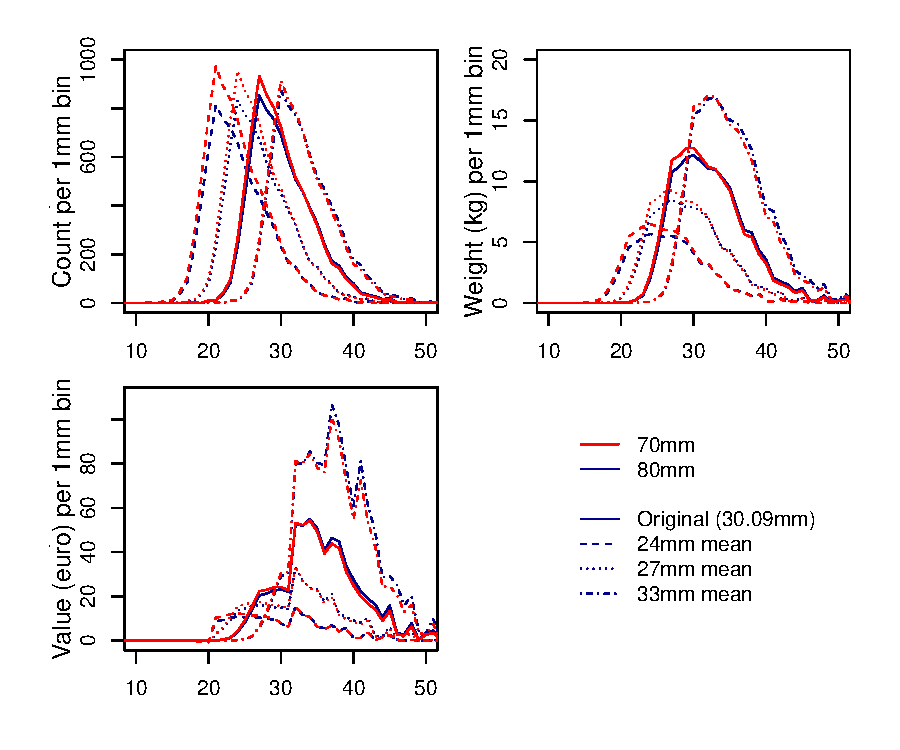
\includegraphics[width=\maxwidth]{figure/split_plots-1} \caption[Simulated counts, weight and value by]{Simulated counts, weight and value by: length class, mesh size and  simulated scenario (24mm mean catch, 27mm mean catch, 30mm mean catch (original), 33mm mean catch).}\label{fig:split_plots}
\end{figure}


\end{knitrout}

Summary table (as in BIM report Table 3)
\begin{knitrout}\footnotesize
\definecolor{shadecolor}{rgb}{0.969, 0.969, 0.969}\color{fgcolor}\begin{kframe}
\begin{alltt}
\hlcom{## calculate the resulting mean sizes per length class}
\hlcom{##apply(count.phaul.sim, 1, FUN = function(z)\{sum(cl.mids * z) / sum(z)\})}
\hlstd{mean.cl.70} \hlkwb{<-} \hlkwd{apply}\hlstd{(count.phaul.sim.70,} \hlnum{1}\hlstd{,} \hlkwc{FUN} \hlstd{=} \hlkwa{function}\hlstd{(}\hlkwc{z}\hlstd{)\{}\hlkwd{sum}\hlstd{(cl.mids} \hlopt{*} \hlstd{z)} \hlopt{/} \hlkwd{sum}\hlstd{(z)\})}
\hlstd{mean.cl.80} \hlkwb{<-} \hlkwd{apply}\hlstd{(count.phaul.sim.80,} \hlnum{1}\hlstd{,} \hlkwc{FUN} \hlstd{=} \hlkwa{function}\hlstd{(}\hlkwc{z}\hlstd{)\{}\hlkwd{sum}\hlstd{(cl.mids} \hlopt{*} \hlstd{z)} \hlopt{/} \hlkwd{sum}\hlstd{(z)\})}

\hlcom{## data frame for predictions}
\hlstd{na.vec} \hlkwb{<-} \hlkwd{rep}\hlstd{(}\hlnum{NA}\hlstd{,} \hlnum{8}\hlstd{)}
\hlstd{sim.order} \hlkwb{<-} \hlkwd{c}\hlstd{(}\hlstr{"original"}\hlstd{,} \hlstr{"mm.33"}\hlstd{,} \hlstr{"mm.27"}\hlstd{,} \hlstr{"mm.24"}\hlstd{)}

\hlstd{pred.df} \hlkwb{<-} \hlkwd{data.frame}\hlstd{(}\hlkwc{Mesh.Size} \hlstd{=} \hlkwd{rep}\hlstd{(}\hlkwd{c}\hlstd{(}\hlnum{70}\hlstd{,} \hlnum{80}\hlstd{),} \hlkwc{each} \hlstd{=} \hlnum{4}\hlstd{),}
                      \hlkwc{Mean.CL} \hlstd{=} \hlkwd{rep}\hlstd{(sim.order,} \hlnum{2}\hlstd{),}
                      \hlkwc{Mean.CL.mesh} \hlstd{=} \hlkwd{c}\hlstd{(mean.cl.70[sim.order], mean.cl.80[sim.order]),}
                      \hlkwc{c.less.mcrs} \hlstd{= na.vec,}
                      \hlkwc{c.greater.mcrs} \hlstd{= na.vec,}
                      \hlkwc{total.catch} \hlstd{= na.vec,}
                      \hlkwc{v.less.mcrs} \hlstd{= na.vec,}
                      \hlkwc{v.greater.mcrs} \hlstd{= na.vec,}
                      \hlkwc{total.value} \hlstd{= na.vec,}
                      \hlkwc{stringsAsFactors} \hlstd{=} \hlnum{FALSE}\hlstd{)}
\hlcom{##}

\hlkwa{for}\hlstd{(i} \hlkwa{in} \hlnum{1}\hlopt{:}\hlkwd{dim}\hlstd{(pred.df)[}\hlnum{1}\hlstd{])\{}
  \hlkwd{print}\hlstd{(i)}
  \hlstd{wt} \hlkwb{<-} \hlkwd{get}\hlstd{(}\hlkwd{paste}\hlstd{(}\hlstr{"wt.phaul.sim."}\hlstd{, pred.df}\hlopt{$}\hlstd{Mesh.Size[i],} \hlkwc{sep} \hlstd{=} \hlstr{""}\hlstd{))}
  \hlstd{value} \hlkwb{<-} \hlkwd{get}\hlstd{(}\hlkwd{paste}\hlstd{(}\hlstr{"value.phaul.sim."}\hlstd{, pred.df}\hlopt{$}\hlstd{Mesh.Size[i],} \hlkwc{sep} \hlstd{=} \hlstr{""}\hlstd{))}
  \hlcom{## catch}
  \hlstd{pred.df}\hlopt{$}\hlstd{c.less.mcrs[i]} \hlkwb{<-} \hlkwd{sum}\hlstd{(wt[pred.df}\hlopt{$}\hlstd{Mean.CL[i], cl.mids} \hlopt{<} \hlnum{20}\hlstd{])}
  \hlstd{pred.df}\hlopt{$}\hlstd{c.less.mcrs[i]} \hlkwb{<-} \hlkwd{round}\hlstd{(pred.df}\hlopt{$}\hlstd{c.less.mcrs[i],} \hlnum{2}\hlstd{)}
  \hlstd{pred.df}\hlopt{$}\hlstd{c.greater.mcrs[i]} \hlkwb{<-} \hlkwd{sum}\hlstd{(wt[pred.df}\hlopt{$}\hlstd{Mean.CL[i], cl.mids} \hlopt{>=} \hlnum{20}\hlstd{])}
  \hlstd{pred.df}\hlopt{$}\hlstd{c.greater.mcrs[i]} \hlkwb{<-} \hlkwd{round}\hlstd{(pred.df}\hlopt{$}\hlstd{c.greater.mcrs[i],} \hlnum{2}\hlstd{)}
  \hlstd{pred.df}\hlopt{$}\hlstd{total.catch[i]} \hlkwb{<-} \hlkwd{sum}\hlstd{(wt[pred.df}\hlopt{$}\hlstd{Mean.CL[i], ])}
  \hlstd{pred.df}\hlopt{$}\hlstd{total.catch[i]} \hlkwb{<-} \hlkwd{round}\hlstd{(pred.df}\hlopt{$}\hlstd{total.catch[i],} \hlnum{2}\hlstd{)}
  \hlcom{## value}
  \hlstd{pred.df}\hlopt{$}\hlstd{v.less.mcrs[i]} \hlkwb{<-} \hlkwd{sum}\hlstd{(value[pred.df}\hlopt{$}\hlstd{Mean.CL[i], cl.mids} \hlopt{<} \hlnum{20}\hlstd{])}
  \hlstd{pred.df}\hlopt{$}\hlstd{v.less.mcrs[i]} \hlkwb{<-} \hlkwd{round}\hlstd{(pred.df}\hlopt{$}\hlstd{v.less.mcrs[i],} \hlnum{2}\hlstd{)}
  \hlstd{pred.df}\hlopt{$}\hlstd{v.greater.mcrs[i]} \hlkwb{<-} \hlkwd{sum}\hlstd{(value[pred.df}\hlopt{$}\hlstd{Mean.CL[i], cl.mids} \hlopt{>=} \hlnum{20}\hlstd{])}
  \hlstd{pred.df}\hlopt{$}\hlstd{v.greater.mcrs[i]} \hlkwb{<-} \hlkwd{round}\hlstd{(pred.df}\hlopt{$}\hlstd{v.greater.mcrs[i],} \hlnum{2}\hlstd{)}
  \hlstd{pred.df}\hlopt{$}\hlstd{total.value[i]} \hlkwb{<-} \hlkwd{sum}\hlstd{(value[pred.df}\hlopt{$}\hlstd{Mean.CL[i], ])}
  \hlstd{pred.df}\hlopt{$}\hlstd{total.value[i]} \hlkwb{<-} \hlkwd{round}\hlstd{(pred.df}\hlopt{$}\hlstd{total.value[i],} \hlnum{2}\hlstd{)}
\hlstd{\}}
\end{alltt}
\begin{verbatim}
## [1] 1
## [1] 2
## [1] 3
## [1] 4
## [1] 5
## [1] 6
## [1] 7
## [1] 8
\end{verbatim}
\end{kframe}
\end{knitrout}

\begin{landscape}
\begin{kframe}
\begin{alltt}
\hlkwd{library}\hlstd{(xtable)}
\hlkwd{print}\hlstd{(}\hlkwd{xtable}\hlstd{(pred.df,} \hlkwc{digits} \hlstd{=} \hlnum{2}\hlstd{,} \hlkwc{align} \hlstd{=} \hlstr{"lccccccccc"}\hlstd{),} \hlkwc{include.rownames} \hlstd{=} \hlnum{FALSE}\hlstd{)}
\end{alltt}
\end{kframe}% latex table generated in R 3.2.2 by xtable 1.7-4 package
% Thu Sep 24 16:08:30 2015
\begin{table}[ht]
\centering
\begin{tabular}{ccccccccc}
  \hline
Mesh.Size & Mean.CL & Mean.CL.mesh & c.less.mcrs & c.greater.mcrs & total.catch & v.less.mcrs & v.greater.mcrs & total.value \\ 
  \hline
70.00 & original & 29.96 & 0.02 & 152.80 & 152.82 & -0.00 & 628.79 & 628.79 \\ 
  70.00 & mm.33 & 32.96 & 0.00 & 200.60 & 200.60 & 0.00 & 1113.07 & 1113.07 \\ 
  70.00 & mm.27 & 26.97 & 0.25 & 112.89 & 113.14 & -0.05 & 353.73 & 353.68 \\ 
  70.00 & mm.24 & 23.97 & 3.46 & 77.50 & 80.96 & -0.69 & 190.95 & 190.26 \\ 
  80.00 & original & 30.23 & 0.02 & 150.65 & 150.67 & -0.00 & 648.12 & 648.12 \\ 
  80.00 & mm.33 & 33.23 & 0.00 & 206.10 & 206.10 & 0.00 & 1187.36 & 1187.36 \\ 
  80.00 & mm.27 & 27.23 & 0.20 & 106.90 & 107.11 & -0.04 & 350.37 & 350.33 \\ 
  80.00 & mm.24 & 24.24 & 2.78 & 70.86 & 73.65 & -0.56 & 182.10 & 181.55 \\ 
   \hline
\end{tabular}
\end{table}

\end{landscape}

\bibliography{../../../../misc/epif_bibliography}
\bibliographystyle{../../../../misc/cjfas}
\end{document}

